\documentclass[11pt]{article}
\usepackage[T1]{fontenc}
\usepackage{lmodern}
\usepackage[margin=1.05in]{geometry}
\usepackage{amsmath,amssymb,amsthm,mathtools}
\usepackage{microtype}
\usepackage{enumitem}
\usepackage{booktabs,array}
\usepackage{tikz}
\usetikzlibrary{arrows.meta,positioning,calc}
\usepackage[nottoc,notlof,notlot,notindex]{tocbibind}
\usepackage{hyperref}
\hypersetup{colorlinks=true,linkcolor=blue!45!black,citecolor=blue!45!black,urlcolor=blue!45!black,pdftitle={Baumslag--Solitar-free one-relator groups are hyperbolic},pdfauthor={OpenAI}}
\newtheorem{theorem}{Theorem}[section]
\newtheorem{lemma}[theorem]{Lemma}
\newtheorem{proposition}[theorem]{Proposition}
\newtheorem{corollary}[theorem]{Corollary}
\theoremstyle{definition}
\newtheorem{definition}[theorem]{Definition}
\newtheorem{remark}[theorem]{Remark}
\numberwithin{equation}{section}
\setcounter{tocdepth}{2}
\setlength{\emergencystretch}{1.5em}
\title{Baumslag--Solitar-free one-relator groups\\are hyperbolic}
\author{OpenAI}
\date{September 25, 2026}
\begin{document}
\maketitle
\begin{abstract}
We prove Gersten's conjecture: every finitely generated one-relator group
containing no subgroup isomorphic to a Baumslag--Solitar group
$\operatorname{BS}(m,n)$, for nonzero integers $m,n$, is word-hyperbolic.
\end{abstract}
\tableofcontents
\section{Introduction}

A single defining relation can produce very different geometries.
The Baumslag--Solitar groups
\[
 \operatorname{BS}(m,n)
   =\langle a,t\mid ta^mt^{-1}=a^n\rangle,
 \qquad m,n\in\mathbb Z\setminus\{0\},
\]
are the basic obstructions to hyperbolicity among one-relator groups.
Gersten asked whether they are the only subgroup obstructions
\cite[p.~228]{Gersten1992Problems}.
We prove the following statement, resolving Gersten's conjecture positively.
Here $F(X)$ denotes the free group on $X$, and
$\langle X\mid r\rangle$ is its quotient by the normal closure of $r$.

\begin{theorem}\label{thm:main}
Let $X$ be a finite set and let $r\in F(X)$. If the one-relator group
$G=\langle X\mid r\rangle$ contains no subgroup isomorphic to
$\operatorname{BS}(m,n)$ for any nonzero integers $m,n$, then $G$ is
word-hyperbolic.
\end{theorem}

The parameters in this statement may have either sign. In particular,
the hypothesis excludes $\operatorname{BS}(1,1)=\mathbb Z^2$.
We call a group with this exclusion \emph{Baumslag--Solitar-free}.
The customary formulation excluding every $\operatorname{BS}(1,n)$,
for every nonzero integer $n$, is equivalent: every Baumslag--Solitar group contains
one of these groups \cite[Lemma~2.10]{GardamKielakLogan2025Algebraically}.
Theorem~\ref{thm:main} includes trivial relators and proper powers; it
has no torsion-free hypothesis.

We use \emph{free-by-cyclic} in the subgroup-closed sense: a group $H$
fits into an exact sequence
\[
1\longrightarrow K\longrightarrow H\longrightarrow Q\longrightarrow1
\]
with $K$ free of possibly infinite rank and $Q\leq\mathbb Z$, possibly
trivial. Kielak--Linton recall Wise's Conjecture~17.8 that every
hyperbolic one-relator group is virtually free-by-cyclic and prove the
conclusion under the additional hypothesis of virtual compact
specialness \cite[Section~1.1 and Corollary~1.3]{KielakLinton2024Virtually}.
The companion theorem \cite[Theorem~1.1]{OpenAIVirtualSpecialness}
provides that hypothesis. Combining it with Theorem~\ref{thm:main}
gives the Baumslag--Solitar-free form in
Corollary~\ref{cor:free-by-cyclic}, together with a finite-index
embedding into a free-by-$\mathbb Z$ group with finitely generated
free kernel.

\subsection{Earlier work and the remaining step}

The classical theory already separates the torsion case from the
main difficulty. Magnus's Freiheitssatz identifies free subgroups
generated by suitable proper subsets of a one-relator generating set
\cite{Magnus1930}. Newman's spelling theorem for proper-power relators
gives a Dehn algorithm and hence hyperbolicity
\cite[Theorem~3]{Newman1968}; see also the proof in
\cite[Theorem~4]{McCoolSchupp1973}. Thus the new hyperbolicity assertion
concerns non-power relators, although Theorem~\ref{thm:main} includes
all relators. The Freiheitssatz makes an inductive approach possible:
a Magnus splitting has a smaller one-relator vertex group and free
edge groups. The geometric form of the
Magnus--Moldavanskii--Masters hierarchy, developed by Linton, realizes
these splittings through domains in cyclic covers
\cite[Sections~1.1--1.2 and~4]{LintonHierarchies2025}.
We use that construction in Section~\ref{mag:section}, with the domain
and complexity arguments given in the form needed here.

Several recent results identify substantial classes where this
induction preserves hyperbolicity. Louder and Wilton characterized
negative immersions for one-relator presentation complexes by
primitivity rank greater than two
\cite[Theorem~1.3]{LouderWilton2022NegativeImmersions}.
Here the primitivity rank of a relator $r$ is the least rank of a
subgroup of $F(X)$ containing $r$ in which $r$ is not part of a free
basis, with value $\infty$ if no such subgroup exists.
Their subgroup theorem excludes Baumslag--Solitar subgroups in this
class, and their subsequent work establishes uniform negative
immersions and coherence
\cite[Corollary~1.8]{LouderWilton2022NegativeImmersions}
\cite[Theorems~A and~C]{LouderWilton2024UniformNegativeImmersions}.
Linton then proved hyperbolicity and virtual specialness for groups
with negative immersions
\cite[Theorem~7.2]{LintonHierarchies2025}.
His later characterization says that a finitely generated one-relator
group is both hyperbolic and locally quasiconvex precisely when its
relator has primitivity rank different from two
\cite[Theorem~1.4]{Linton2025MappingToriSubgroups}.
Local quasiconvexity means that every finitely generated subgroup is
quasiconvex. This characterization does not settle hyperbolicity
alone for Baumslag--Solitar-free groups whose relator has primitivity
rank two.

Linton's hierarchy criterion makes the remaining obstruction more
specific: a one-relator hierarchy is quasiconvex with hyperbolic
ambient group if and only if it is $\mathbb Z$-stable and the group is
Baumslag--Solitar-free
\cite[Theorem~7.1]{LintonHierarchies2025}.
The stability hypothesis controls the persistence of noncyclic
intersections along the hierarchy; it is an additional condition,
not a consequence supplied by that criterion.
A complementary reduction to primitive-extension groups isolates a
particular class of two-generator one-relator groups in which to
settle the conjecture
\cite[Theorem~5.6 and Corollary~5.7]{LintonHyperbolic2026}.
For a broader historical account, see
\cite{LintonNybergBrodda2025Survey}.

The geometric issue is expansion in a graph of groups. The
Bestvina--Feighn combination theorem makes annular flaring a sufficient
condition for hyperbolicity when the vertex and edge data satisfy the
required geometric hypotheses
\cite[Theorem~1.2]{BestvinaFeighn1996Addendum}.
We use the algebraic annular formulation in
\cite[Theorem~4.5]{Kapovich1999NonQuasiconvexity}.
For mapping tori of free-group automorphisms, Brinkmann proved that
the absence of periodic conjugacy classes forces expansion and
hyperbolicity \cite{Brinkmann2000HyperbolicAutomorphisms}.
Mutanguha extended the hyperbolicity criterion to ascending HNN
extensions of finite-rank free groups: they are hyperbolic exactly
when they contain no Baumslag--Solitar subgroup
\cite[Theorem~6.7]{Mutanguha2021}.
His expanding relative immersions, iterated pullbacks, and annular
arguments supply important precedents for treating persistent
intersections \cite[Theorem~4.5 and Sections~5--6]{Mutanguha2021}.
The combination theorem here permits both free edge subgroups to be
proper in a hyperbolic vertex group, under the intersection and rank
hypotheses below.

\subsection{The combination argument}

Our main technical result is a combination theorem for a restricted
class of HNN extensions of torsion-free hyperbolic groups
(Theorem~\ref{ann:combination}). The Magnus construction reduces the problem to a one-relator vertex
group of smaller complexity and finitely generated free edge groups.
Once the vertex group is hyperbolic, Linton's quasiconvexity theorem gives
quasiconvex edge groups. Two further intersection properties are needed:
conjugates of the edge groups have noncyclic intersection only in one
specified double coset, and their overlap subgroups satisfy a strong
reduced-rank inequality.
Collins's intersection theorem and Linton's strong-inertia result supply
these properties for the Magnus splittings used here
\cite{Collins2008Conjugates,LintonHierarchies2025}.
The combination theorem shows that the absence of Baumslag--Solitar
subgroups forces annular flaring under precisely these hypotheses.

We prove flaring by contradiction, using free-group currents:
invariant measures on pairs of distinct boundary points
\cite{KapovichCurrents2006}.
Long nonflaring annuli give a nonzero stationary current for which
almost every line can be transferred across successive edges of the
Bass--Serre tree.
The stabilizers of increasingly long tree paths are represented by
finite labeled core graphs. The rank inequality bounds the number of
edges after degree-two vertices are suppressed; it does not bound
their label lengths. Along a subsequence, the edges with bounded
labels form one fixed graph, called the small subgraph. Its noncyclic
components determine finitely many maximal subgroup carriers for
persistent path stabilizers. A return along a carrier induces an
atoroidal automorphism, with no nontrivial periodic conjugacy class.
Brinkmann's expansion theorem then forces the set of carrier lines
to have zero current mass.

Zero mass does not exclude a carrier line from the closed support of
the current. This distinction is the main issue in
Section~\ref{exp:section}. Starting with a putative carrier line in
the support, we transport a positive-mass cylinder along expanding
carrier returns.
If this transport continues to follow the prescribed carrier,
recentering and compactness concentrate positive mass on its
zero-mass line set. If it fails, the stabilizers of the competing
actual tree path and the prescribed path have at most cyclic
intersection. A sufficiently long overlap consequently follows a
periodic axis of uniformly bounded primitive period.
Recentering these overlaps puts a periodic line in the support.
We reuse this same failure mechanism to exclude periodic support
lines: pulling the overlap back along the carrier return preserves
enough whole periods to identify the failure axis with the original
periodic trajectory, contradicting the competing path choices.
Counting whole periods is essential because inverse automorphisms
can enlarge primitive period lengths.

It follows that no support line lies in the small subgraph and that
every support line has irrational endpoints. The bounded graph
complexity now leaves only finitely many rays admitting two
different pasts. Transfer permutes their finitely many endpoint
orbits under the free edge group. A return at one of these endpoints
supplies infinitely many disjoint translates of a fixed positive-mass
set inside a compact set,
contradicting local finiteness of the current. This proves the
restricted combination theorem; the geometric Magnus induction
then proves Theorem~\ref{thm:main}.

\subsection{Magnus subgraphs}

We also record the geometric subgroup conclusion in the scope needed
by the induction. A \emph{circuit} in a graph is a map from a subdivided
circle; it is \emph{immersed} when its edge path has no backtracking,
including at the closing point. A nontrivial element is a
\emph{non-power} if it is not $u^k$ with $|k|\geq2$.

\begin{theorem}\label{thm:magnus}
Let $\Gamma$ be a finite connected graph, and let
$\lambda:S^1\to\Gamma$ be a nontrivial immersed circuit representing a
non-power in $\pi_1\Gamma$. Attach a $2$-cell along $\lambda$, obtaining
$Y$. If $\pi_1Y$ is Baumslag--Solitar-free, then, for every connected
subgraph $S\subseteq\Gamma$ with $\lambda(S^1)\nsubseteq S$, the map
\[
 \pi_1S\longrightarrow\pi_1Y
\]
is injective and its image is quasiconvex.
\end{theorem}

A choice of basepoint paths changes these subgroups only by conjugacy.
Such an $S$ is called a \emph{Magnus subgraph}. Its injectivity follows
from the Freiheitssatz. Once Theorem~\ref{thm:main} gives ambient
hyperbolicity, its quasiconvexity follows from Linton's theorem that
Magnus subgroups of hyperbolic one-relator groups are quasiconvex
\cite[Theorem~4.7]{LintonHyperbolic2026}.
We prove the graph-to-basis identification explicitly in
Lemma~\ref{mag:graph-magnus}. The same quasiconvexity theorem supplies the
quasiconvex edge groups at each inductive step, so the induction needs
only to establish hyperbolicity of the smaller vertex group.

\subsection{Structure of the proof}

Sections~\ref{pre:section}--\ref{ray:section} prove the restricted
combination theorem. Section~\ref{ann:section} states its hypotheses and
converts nonflaring annuli into a bounded bilateral sequence of
currents. Section~\ref{stat:section} removes atoms and obtains a
stationary current with well-defined transfers on a conull set.
Sections~\ref{car:section} and~\ref{exp:section} construct the finite
carriers and exclude periodic support lines. Section~\ref{ray:section}
finishes the measure contradiction. Finally, Section~\ref{mag:section}
constructs a decreasing Magnus induction and proves
Theorems~\ref{thm:main} and~\ref{thm:magnus}.
Section~\ref{sec:free-by-cyclic} derives the virtual free-by-cyclic
consequence and records the corresponding ascending-HNN consequence
of the companion theorem.

\section{Intersections, cyclic commensurators, and rank bounds}
\label{pre:section}

We need three preliminary tools. The first controls intersections of
quasiconvex subgroups. The second produces an embedded Baumslag--Solitar
subgroup from a tree action. The third bounds the total reduced rank of
a family of conjugate intersections.

\subsection{Quasiconvex intersections}

All word metrics come from finite generating sets. A group is
\emph{word-hyperbolic} if geodesic triangles in a Cayley graph are
uniformly thin: each side lies in a fixed neighborhood of the other two.
A subgroup of a
hyperbolic group is \emph{quasiconvex} if every geodesic between its elements
lies in a fixed neighborhood of the subgroup. We use the Morse lemma and
its usual consequences: quasiconvex subgroups are finitely generated and
quasi-isometrically embedded, these two properties characterize
quasiconvexity, and infinite cyclic subgroups are quasiconvex. In particular,
quasiconvexity is transitive between hyperbolic groups, since
quasi-isometric embeddings compose. For these background facts, see
\cite[Theorem~III.H.1.7, Corollary~III.$\Gamma$.3.6(2), and
Corollary~III.$\Gamma$.3.10(1)]{BridsonHaefliger1999}.
For a subset \(Q\) of a hyperbolic
group, write \(\Lambda Q\) for its accumulation set in the boundary.

\begin{lemma}[Quasiconvex intersections]
\label{pre:quasiconvex-intersection}
Let \(K,L\) be quasiconvex subgroups of a finitely generated hyperbolic
group \(H\). Then \(K\cap L\) is quasiconvex and
\[
  \Lambda(K\cap L)=\Lambda K\cap\Lambda L.
\]
The same assertions hold for any finite family of quasiconvex subgroups.
\end{lemma}

\begin{proof}
First observe that, for fixed subgroups \(K,L\) of any finitely generated
group and \(R\geq 0\), there is a constant \(D\) such that
\begin{equation}
  N_R(K)\cap N_R(L)\subseteq N_D(K\cap L).
  \label{pre:neighborhood-intersection}
\end{equation}
Indeed, if \(x\) belongs to the left side, choose \(k\in K\) and \(l\in L\)
within distance \(R\) of \(x\). The element \(d=k^{-1}l\) lies in the finite
ball of radius \(2R\). For each value \(d\) that occurs, fix one pair
\(k_d\in K,l_d\in L\) with \(k_d^{-1}l_d=d\). Then
\[
  z=kk_d^{-1}=ll_d^{-1}\in K\cap L,
  \qquad d(x,z)\leq R+|k_d|.
\]
Taking a maximum over the finitely many \(d\) proves
\eqref{pre:neighborhood-intersection}.

A geodesic with endpoints in \(K\cap L\) lies in fixed neighborhoods of
both \(K\) and \(L\), so \eqref{pre:neighborhood-intersection} proves
quasiconvexity of their intersection.

Now let \(\xi\in\Lambda K\cap\Lambda L\). Quasiconvexity and limits of
geodesic segments show that a ray from the identity to \(\xi\) lies in
bounded neighborhoods of both subgroups. Applying
\eqref{pre:neighborhood-intersection} along the ray gives a sequence in
\(K\cap L\) converging to \(\xi\). Thus
\(\xi\in\Lambda(K\cap L)\). The reverse inclusion is immediate, and
induction gives the finite-family assertions.
These facts also appear in
\cite[Lemmas~2.6 and~2.7]{GitikMitraRipsSageev1998}.
\end{proof}

\begin{lemma}[Finite double-coset lists]
\label{pre:double-coset-finiteness}
Let \(K,L\) be quasiconvex subgroups of a finitely generated hyperbolic
group \(H\). There are only finitely many double cosets \(KgL\) such that
\(K\cap gLg^{-1}\) contains an infinite-order element. If \(H\) is
torsion-free, there are therefore only finitely many such double cosets
with nontrivial intersection.
\end{lemma}

\begin{proof}
Suppose that \(c\in K\cap gLg^{-1}\) has infinite order. Its two fixed
boundary points belong to both \(\Lambda K\) and \(\Lambda(gL)\): use the
sequences \(c^n\in K\) and \(c^ng\in gL\), for positive and negative \(n\).
A geodesic line between those points lies in a uniformly bounded
neighborhood of each of \(K\) and \(gL\). To see the uniformity, a
\(q\)-quasiconvex set contains finite geodesics between its points within
distance \(q\); passing to limits, and then comparing geodesics with the
same ideal endpoints, increases this bound by a constant depending only
on the hyperbolicity constant. The quasiconvexity constant of \(gL\)
equals that of \(L\).

At any point of this line choose nearby vertices \(k\in K\) and
\(gl\in gL\). Their distance is bounded by a constant depending only on
the two quasiconvexity constants and the hyperbolicity constant. Hence
\(k^{-1}gl\in KgL\) lies in a fixed finite ball. Every double coset under
consideration meets that ball, proving finiteness.
\end{proof}

The qualification about infinite-order elements is necessary in groups
with torsion. For example, the central subgroup \(C_2\) of the hyperbolic
group \(F_2\times C_2\) has nontrivial intersection with every conjugate,
but there are infinitely many \(C_2\)-double cosets.

For later applications to cosets, note also that
\[
  \Lambda(gL)=\Lambda(gLg^{-1}).
\]
Indeed, right multiplication by the fixed element \(g^{-1}\) moves each
point of \(gL\) a bounded distance.

\subsection{Commensuration in a tree action}

Two subgroups are \emph{commensurable} if their intersection has finite
index in both. For a subgroup \(C\leq H\), its commensurator is
\[
  \operatorname{Comm}_H(C)
  =\{h\in H: C\text{ and }hCh^{-1}\text{ are commensurable}\}.
\]
This is a subgroup. We first deduce the cyclic case directly from the
double-coset lemma.

\begin{lemma}
\label{pre:cyclic-commensurator}
If \(C\) is an infinite cyclic subgroup of a hyperbolic group \(H\), then
\(C\) has finite index in \(\operatorname{Comm}_H(C)\).
If \(H\) is torsion-free, this commensurator is infinite cyclic.
\end{lemma}

\begin{proof}
The subgroup \(C\) is quasiconvex. By
Lemma~\ref{pre:double-coset-finiteness}, its commensurator meets only
finitely many double cosets \(CgC\). For a representative \(g\) in the
commensurator, \(CgC\) is a union of
\([C:C\cap g^{-1}Cg]\) left \(C\)-cosets, a finite number. Thus the
commensurator is virtually cyclic. A torsion-free virtually cyclic group
is cyclic, giving the last assertion.
\end{proof}

All tree actions below are actions on simplicial trees without
inversions. An element is \emph{elliptic} if it fixes a vertex and
\emph{tree-hyperbolic} if it translates a bi-infinite geodesic.
We will need an embedded Baumslag--Solitar group, rather than just a
power-conjugacy relation. The following normal-form argument provides it.

\begin{lemma}[Graphs of cyclic groups]
\label{pre:gbs-subgroup}
Let \(Q\) be a finitely generated noncyclic group acting on a simplicial
tree without inversions. If every vertex and edge stabilizer is infinite
cyclic, then \(Q\) contains a subgroup isomorphic to \(BS(m,n)\) for some
nonzero integers \(m,n\).
\end{lemma}

\begin{proof}
Choose a vertex \(v\) and a finite symmetric generating set \(S\) of \(Q\).
The union of all \(Q\)-translates of the finite subtree
\[
  D=\bigcup_{s\in S}[v,sv]
\]
is connected: its segments connect the vertices in the orbit \(Qv\)
according to the Cayley graph of \(Q\). This union is exactly the convex
hull of \(Qv\), because its segments join orbit points. Restricting the
action to this hull gives a finite quotient, since every edge orbit has
a representative in \(D\). The retained vertex and edge stabilizers are
unchanged. Bass--Serre theory therefore realizes \(Q\) as the fundamental
group of a finite connected graph of infinite cyclic groups.

Collapse any non-loop edge whose map to one endpoint group is onto.
Such a collapse preserves the fundamental group and leaves a graph of
infinite cyclic groups. After finitely many collapses, every remaining
non-loop edge has both inclusion indices greater than one.

If a loop remains, the subgraph consisting of that loop and its vertex
has fundamental group
\[
  \langle x,t\mid t x^m t^{-1}=x^n\rangle=BS(m,n),
  \qquad m,n\neq 0.
\]
Its fundamental group injects into \(Q\) by the graph-of-groups normal
form theorem.

If a non-loop edge remains, its two-vertex subgraph likewise injects and
has fundamental group
\[
  \langle x,y\mid x^m=y^n\rangle,
  \qquad |m|,|n|>1.
\]
The element \(z=x^m=y^n\) is central and has infinite order. Modulo
\(\langle z\rangle\), this group is \(C_{|m|}*C_{|n|}\), in which the image
of \(xy\) has infinite order by free-product normal form. Thus the
commuting elements \(z\) and \(xy\) generate an embedded
\(\mathbb Z^2=BS(1,1)\).

Finally, if no edge remains, the graph has one vertex and \(Q\) is
cyclic, contrary to the hypothesis. This exhausts the possibilities.
\end{proof}

\begin{lemma}[Elliptic commensuration]
\label{pre:elliptic-commensurator}
Suppose that \(G\) acts on a simplicial tree \(\mathcal T\) without
inversions, with torsion-free hyperbolic vertex stabilizers. If an
infinite-order elliptic element \(a\in G\) has its cyclic subgroup
commensurated by a tree-hyperbolic element \(g\in G\), then \(G\) contains
a subgroup isomorphic to \(BS(m,n)\) for some nonzero integers \(m,n\).
\end{lemma}

\begin{proof}
Set \(L=\langle a,g\rangle\) and choose a vertex \(v\) fixed by \(a\).
Every element of \(L\) commensurates \(\langle a\rangle\). For each
\(h\in L\), commensurability supplies nonzero integers \(r,s\) with
\(a^r=ha^sh^{-1}\); hence a nonzero power of \(a\) fixes \(hv\).
A common multiple of finitely many such powers fixes any prescribed
finite subset of \(Lv\), and therefore fixes its convex hull pointwise.
It follows that every finite subtree of
\(\mathcal T_L=\operatorname{Hull}(Lv)\) is fixed by a nonzero power of
\(a\).

Let \(x\) be a vertex of \(\mathcal T_L\), and choose \(N>0\) with
\(a^N\in L_x\). Every element of \(L_x\) commensurates
\(\langle a^N\rangle\), now a subgroup of the vertex stabilizer \(G_x\).
Thus
\[
  \langle a^N\rangle
  \leq L_x
  \leq \operatorname{Comm}_{G_x}(\langle a^N\rangle).
\]
Lemma~\ref{pre:cyclic-commensurator} makes the last group infinite cyclic,
so \(L_x\) is infinite cyclic as well. Each edge stabilizer of
\(\mathcal T_L\) contains a nonzero power of \(a\) and is a subgroup of a
vertex stabilizer in \(L\); it too is infinite cyclic.

The group \(L\) is noncyclic. Otherwise, writing \(a=c^r\) and \(g=c^s\)
in a cyclic group, translation lengths would give
\(\ell(a)=|r|\ell(c)=0\) and hence \(\ell(g)=0\), contrary to
tree-hyperbolicity of \(g\). Apply Lemma~\ref{pre:gbs-subgroup} to the
action of the finitely generated group \(L\) on \(\mathcal T_L\).
\end{proof}

\subsection{Strong inertia in free groups}

We now formulate the rank estimate that will control noncyclic
intersections. For a finitely generated free group \(K\), put
\[
  \bar r(K)=\max\{\operatorname{rk}(K)-1,0\}.
\]
Strong inertia bounds the sum of reduced ranks of all conjugate
intersections; see
\cite{LintonHierarchies2025}.

\begin{definition}
\label{pre:strong-inertia-definition}
A finitely generated subgroup \(E\) of a finitely generated free group
\(P\) is \emph{strongly inert} if, for every finitely generated subgroup
\(S\leq P\),
\begin{equation}
  \sum_{SpE\in S\backslash P/E}
  \bar r(E\cap p^{-1}Sp)\leq\bar r(S).
  \label{pre:strong-inertia-inequality}
\end{equation}
The summands are independent of the chosen double-coset representatives.
Only finitely many intersections are nontrivial, by
Lemma~\ref{pre:double-coset-finiteness}.
\end{definition}

\begin{corollary}
\label{pre:cyclic-off-diagonal}
Let \(P\) be a finitely generated free group and \(E\leq P\) a strongly
inert subgroup. If \(g\in P\setminus E\), then
\(E\cap gEg^{-1}\) is trivial or cyclic.
\end{corollary}

\begin{proof}
Apply \eqref{pre:strong-inertia-inequality} with \(S=E\).
The identity double coset contributes \(\bar r(E)\), so all other
nonnegative summands vanish.
\end{proof}

\section{Annuli and currents for a restricted HNN extension}
\label{ann:section}

We now isolate the combination statement used in the Magnus induction.
The restrictions on intersections in its hypotheses will provide a uniform
bound on the ranks of path stabilizers.  In this section we establish that
failure of hyperbolicity produces a bounded, nonzero trajectory of free-group
currents.  The subsequent sections rule out that trajectory and thereby
complete the combination argument.

\begin{theorem}[Restricted combination theorem]
\label{ann:combination}
Let $H$ be a torsion-free word-hyperbolic group, let $A,B\leq H$ be
finitely generated free quasiconvex subgroups, and let $\phi\colon A\to B$
be an isomorphism.  Set
\[
 G=\langle H,t\mid tat^{-1}=\phi(a)\ (a\in A)\rangle,
 \qquad P=A,\qquad I=A\cap B,\qquad J=t^{-1}It\leq P.
\]
Assume the following two conditions.
\begin{enumerate}[label=\textup{(\roman*)}]
\item For $M,N\in\{A,B\}$ and $g\in H$, the intersection
      $M\cap gNg^{-1}$ is at most cyclic unless $g\in MN$.
\item The groups $I,J$ are finitely generated, and each $E\in\{I,J\}$
      satisfies
      \begin{equation}
      \sum_{SpE\in S\backslash P/E}
        \bar r(E\cap p^{-1}Sp)\leq\bar r(S)
      \qquad\text{for every finitely generated }S\leq P.
      \label{ann:inertia-assumption}
      \end{equation}
\end{enumerate}
If $G$ contains no subgroup isomorphic to $BS(m,n)$ for any nonzero
integers $m,n$, then $G$ is word-hyperbolic.
\end{theorem}

All the intersection restrictions in this statement are hypotheses.
In particular, the assertion concerns a restricted class of HNN
extensions.  We retain the notation of Theorem~\ref{ann:combination}
throughout the combination argument.  Write
\[
 i\colon I\longrightarrow P,\quad i(c)=c,
 \qquad
 j\colon I\longrightarrow P,\quad j(c)=t^{-1}ct,
\]
so that $j(I)=J$.  Fix finite generating sets for $H$ and a free basis
for $P$.  We write $|\cdot|_H$ and $|\cdot|_P$ for the associated based
word lengths.  If $P=1$, then $G=H*\mathbb Z$ is hyperbolic, so we may
assume $P\ne1$ in what follows.

\subsection{Frames and stabilizers of paths}

Let $\mathcal T$ be the Bass--Serre tree of the HNN extension.  The height
homomorphism $G\to\mathbb Z$ sends $t$ to $1$ and $H$ to $0$.  Orient
the canonical edge $e$ from $t^{-1}H$ to $H$, and orient every translate
equivariantly.  Its stabilizer is $P$.  A \emph{frame} for the edge $he$
is the element $h\in G$; changing $h$ to $hp$, with $p\in P$, changes
the coordinates on its stabilizer but not the edge.  A path traverses an
edge positively if it follows this orientation.

\begin{lemma}[Neighboring edges and frames]
\label{ann:frames}
A reduced path in $\mathcal T$ with noncyclic pointwise stabilizer has
constant traversal sign.  The positive successors of $e$ that can occur
in such a path have the form $pte$, with $pI\in P/I$, and the positive
predecessors have the form $pt^{-1}e$, with $pJ\in P/J$.  Their common
stabilizers with $e$ are, respectively,
\[
 pIp^{-1}\quad\text{and}\quad pJp^{-1}.
\]
For a positive successor the coordinate transfer is
$c\mapsto t^{-1}p^{-1}cpt$; for a positive predecessor it is
$c\mapsto tp^{-1}cpt^{-1}$, on the indicated domains.
\end{lemma}

\begin{proof}
Every positively oriented edge leaving $H$ is $ate$ for some $a\in H$;
the possible edges are parametrized by $aB\in H/B$.  Its common
stabilizer with $e$ is $A\cap aBa^{-1}$.  If this intersection is
noncyclic, assumption~\textup{(i)} gives $a\in AB$.  Write $a=pb$ with
$p\in P$ and $b\in B$.  Since $bt=t\phi^{-1}(b)$, the edge $ate$ is
$pte$.  Moreover,
\[
 pte=qte
 \quad\Longleftrightarrow\quad
 t^{-1}q^{-1}pt\in A
 \quad\Longleftrightarrow\quad q^{-1}p\in A\cap B=I.
\]
The common stabilizer is
$P\cap pBp^{-1}=pIp^{-1}$, and conjugating by $(pt)^{-1}$ gives
the stated transfer.

A positive predecessor ending at $t^{-1}H$ is $t^{-1}ae$, with
$aA\in H/A$.  After conjugating its pair stabilizer by $t$, we obtain
$B\cap aAa^{-1}$.  Noncyclicity gives $a\in BA$; writing $a=br$ and
$p=t^{-1}bt\in P$ puts the predecessor in the form $pt^{-1}e$.
Two such edges agree exactly when
\[
 q^{-1}p\in P\cap t^{-1}Pt
 =t^{-1}(B\cap A)t=J.
\]
Their common stabilizer with $e$ is $pJp^{-1}$, and conjugation by
$(pt^{-1})^{-1}$ is the claimed transfer.

At a reversal of traversal sign, the consecutive edge stabilizers, in
the common vertex coordinates, are $M$ and $aMa^{-1}$ for the same
$M\in\{A,B\}$.  The edges are distinct because the path is reduced, so
$a\notin M$.  Assumption~\textup{(i)} makes their intersection at most
cyclic.  A noncyclic stabilizer of the whole path cannot lie in that
intersection.  Thus there are no reversals.
\end{proof}

We call a consecutive positive pair \emph{aligned} when its bridge lies
in the double coset $AB$ in the common vertex coordinates.  Reversing the
traversal gives the corresponding definition for a consecutive negative
pair.  Lemma~\ref{ann:frames} says that every path with noncyclic
stabilizer is aligned after its traversal sign is fixed.

\begin{lemma}[Rank bound for a fixed window]
\label{ann:window-bound}
Fix integers $\ell,r\geq0$.  Consider the positively traversed reduced
paths with edges indexed by $-\ell,\ldots,r$, with edge $0$ equal to $e$,
and with noncyclic pointwise stabilizer.  Then
\begin{equation}
 \sum_{[W]\in P\backslash\{\text{such paths}\}}
       \bar r\bigl(\operatorname{Stab}_G(W)\bigr)
 \leq\bar r(P).
 \label{ann:window-sum}
\end{equation}
Every stabilizer in this sum is finitely generated and free.  In
particular, there are at most $\bar r(P)$ such $P$-orbits.  Equivalently,
the same bound holds for $G$-orbits if the distinguished edge is allowed
to vary.
\end{lemma}

\begin{proof}
Build the fixed window by starting with $e$ and adding one edge at an
endpoint at a time.  The initial stabilizer is $P$.  Suppose $W$ is an
existing representative, $S=\operatorname{Stab}_G(W)\leq P$, and $h$
is a frame at the endpoint edge being extended.  In that frame put
$K=h^{-1}Sh\leq P$.

For a forward extension whose stabilizer is noncyclic,
Lemma~\ref{ann:frames} restricts the next edge to $hpte$, with
$pI\in P/I$.  The action of $S$ on these choices becomes left
multiplication by $K$.  Thus the extension orbits over the orbit of $W$
are indexed by the double cosets $KpI$, and the extended stabilizer is
isomorphic to $K\cap pIp^{-1}$.  Assumption~\textup{(ii)} gives
\[
 \sum_{KpI}\bar r(K\cap pIp^{-1})\leq\bar r(K)=\bar r(S).
\]
For backward extension use $J$ and its separately assumed inequality.
The stabilizers remain finitely generated: in the current edge
coordinates an extension takes the intersection of two finitely generated
subgroups of the finite-rank free group $P$.

The forgetful map from extended windows to the preceding windows is
$P$-equivariant.  Its fiber over the orbit of $W$ is precisely the set of
extensions modulo $S$, which is the double-coset set just considered.
Summing the displayed inequality over the existing representatives
therefore proves the induction step.  Windows with cyclic stabilizer
may be discarded, since extension only decreases a stabilizer.  This
proves~\eqref{ann:window-sum}.  Each noncyclic term contributes at least
one, proving the orbit bound.  Finally,
$\operatorname{Stab}_G(e)=P$, which identifies the two stated orbit sets.
\end{proof}

The shape $(\ell,r)$ is fixed in this lemma; no bound is asserted for the
union of windows of all lengths.  We shall also use the following direct
consequence of the same hypotheses.

\begin{lemma}
\label{ann:distinct-paths}
Two distinct aligned paths of the same fixed window shape with
distinguished edge $e$ and the same traversal sign have at most cyclic
common pointwise stabilizer.
\end{lemma}

\begin{proof}
At their first divergence from the common part, the common stabilizer,
in the shared endpoint frame, lies in
\[
 pEp^{-1}\cap qEq^{-1},\qquad pE\ne qE,
 \qquad E\in\{I,J\}.
\]
This intersection is at most cyclic.  Indeed, apply
\eqref{ann:inertia-assumption} with $S=E$.  The diagonal double coset
already contributes $\bar r(E)$, so every other term has reduced rank
zero.  Since $p^{-1}q\notin E$, the displayed intersection is one of
these off-diagonal intersections up to conjugacy.  If $E$ is cyclic or
trivial, the conclusion is immediate as well.
\end{proof}

\subsection{The algebraic annular-flaring criterion}

We state the external combination theorem with its quantifiers before
passing to limits.  This is important because the width bound in a
sequence of counterexamples will depend on the number of rows.

For a traversal sign $\epsilon\in\{+,-\}$ define the arriving and
departing maps into $H$ by
\[
 f_+(c)=c,\qquad f_-(c)=tct^{-1},\qquad
 l_+(c)=tct^{-1},\qquad l_-(c)=c.
\]
An \emph{algebraic annulus with $2m+1$ rows} consists of signs
$\epsilon_s\in\{+,-\}$ and elements $c_s\in P\setminus\{1\}$ for
$-m\leq s\leq m$, together with bridges $a_s\in H$ for
$-m\leq s<m$, satisfying
\begin{equation}
 f_{\epsilon_s}(c_s)
   =a_s l_{\epsilon_{s+1}}(c_{s+1})a_s^{-1}.
 \label{ann:row-equation}
\end{equation}
Its width is $\max_s|a_s|_H$ and its girth is $|c_0|_P$.  It is
\emph{essential} if a $+,-$ transition has $a_s\notin A$ and a $-,+$
transition has $a_s\notin B$.  There is no restriction at equal-sign
transitions.  It is $\lambda$-\emph{hyperbolic} if
\[
 \max\{|c_{-m}|_P,|c_m|_P\}\geq\lambda|c_0|_P.
\]
All these lengths are based word lengths.

For completeness, these definitions describe an actual reduced tree
path.  Write $f_{\epsilon_s}(c)=u^{-1}cu$ and
$l_{\epsilon_{s+1}}(c)=v^{-1}cv$, where $u,v\in\{1,t^{-1}\}$.
Starting with a frame $h_s$, choose
\begin{equation}
 h_{s+1}=h_su a_sv^{-1}.
 \label{ann:frame-equation}
\end{equation}
The two edges meet at $h_suH=h_{s+1}vH$, and
\eqref{ann:row-equation} gives
$h_sc_sh_s^{-1}=h_{s+1}c_{s+1}h_{s+1}^{-1}$.  Thus a single nontrivial
element fixes the developed path.  The four possible frame multipliers
are
\[
\begin{array}{c|cccc}
 (\epsilon_s,\epsilon_{s+1})&(+,+)&(+,-)&(-,+)&(-,-)\\ \hline
 u a_sv^{-1}&a_st&a_s&t^{-1}a_st&t^{-1}a_s.
\end{array}
\]
At the two reversing transitions the consecutive geometric edges agree
exactly when $a_s\in A$ or $a_s\in B$, respectively.  Essentiality is
therefore exactly absence of backtracking.

\begin{theorem}[Algebraic annular flaring]
\label{ann:external-flaring}
Let $H$ be word-hyperbolic, let $A,B\leq H$ be finitely generated,
and let $\phi:A\to B$ be an isomorphism such that both attaching
maps $A\to H$ are quasi-isometric embeddings. Set
$G=\langle H,t\mid tat^{-1}=\phi(a),\ a\in A\rangle$.
Then $G$ is word-hyperbolic if there exist $\lambda>1$ and an integer
$m\geq1$ such that, for every $\rho>0$, there is $h(\rho)$ for which
every essential algebraic annulus as defined above, with $2m+1$ rows,
width at most $\rho$, and girth at least $h(\rho)$, is
$\lambda$-hyperbolic.
\end{theorem}

This is the algebraic formulation of the Bestvina--Feighn combination
theorem in \cite[Theorem~1.2]{BestvinaFeighn1996Addendum}; we use its explicit
annular statement in \cite[Definitions~4.1--4.4 and Theorem~4.5]{Kapovich1999NonQuasiconvexity}.
The latter numbers refer to the arXiv version of that paper.  Our
$2m+1$ counts the successive edge groups, including both ends.  The
criterion applies here because $A$ and $B$ are quasiconvex in the
hyperbolic group $H$.

\begin{lemma}[Counterannuli at a fixed length]
\label{ann:counterannuli}
If $G$ is not hyperbolic, then for every $m\geq1$ there is a sequence
of essential annuli with $2m+1$ rows whose signs and bridges are fixed
throughout the sequence, such that
\[
 |c_0|_P\longrightarrow\infty,
 \qquad |c_{-m}|_P,|c_m|_P<2|c_0|_P.
\]
For each fixed $s\in[-m,m]$, the ratios $|c_s|_P/|c_0|_P$ are bounded.
The bounds and the fixed bridge tuple may depend on $m$.
\end{lemma}

\begin{proof}
Negate Theorem~\ref{ann:external-flaring} with $\lambda=2$.  For each
$m$ there is a finite width bound $\rho_m$ and counterannuli of
arbitrarily large girth with width at most $\rho_m$.  Choose such a
sequence with girth tending to infinity.  There are finitely many sign
tuples and finitely many bridge tuples of this fixed length and width,
so a subsequence fixes both tuples.

The maps $f_\epsilon,l_\epsilon$ are quasi-isometric embeddings.  The
row equation, with the bridges now fixed, gives constants $L\geq1$ and
$D\geq0$ such that
\[
 |c_{s+1}|_P\leq L|c_s|_P+D,
 \qquad |c_s|_P\leq L|c_{s+1}|_P+D
\]
at every row of this fixed sequence.  Iterating from row $0$ bounds all
the indicated ratios, since $|c_0|_P\to\infty$.
\end{proof}

\subsection{Currents and induction along an injection}

Let $F$ be a nontrivial finite-rank free group with a fixed free basis,
and let $T_F$ be its Cayley tree.  The space
\[
 \partial^2F=(\partial F\times\partial F)\setminus\{(\xi,\xi):
 \xi\in\partial F\}
\]
parametrizes oriented geodesic lines: $(\xi,\zeta)$ is directed from
$\xi$ to $\zeta$.  For a finite nondegenerate oriented segment $\gamma$
in $T_F$, let $\operatorname{Cyl}_F(\gamma)$ be the set of lines
containing it with that orientation.  These compact-open cylinders
form a basis for the topology.  Let $\mathcal L_F(v)$ be the set of
oriented lines passing through the vertex $v$.  It is a finite disjoint
union of the cylinders on edges directed out of $v$, hence is compact
open.

A \emph{current} on $F$ is a nonnegative, $F$-invariant, flip-invariant
Radon measure on $\partial^2F$.  Denote its cone by
$\operatorname{Curr}(F)$ and give it the topology of convergence on
compact-open cylinders.  Its norm is
\begin{equation}
 \|\mu\|_F=\frac12\mu\bigl(\mathcal L_F(1)\bigr).
 \label{ann:current-norm}
\end{equation}
This norm is additive on the cone.  It vanishes only on the zero
current, since translates of $\mathcal L_F(1)$ cover $\partial^2F$.
We omit the subscript when the group and basis are clear.

For $w\in F\setminus\{1\}$, the \emph{counting current} $\eta_w$
is the sum of point masses at the two orientations of the translates
of the axis of $w$, indexed by $F/\langle w\rangle$.  Indexing by
$\langle w\rangle$ retains the multiplicity when $w$ is a proper
power.  Directly counting the translated axes through $1$ gives
\begin{equation}
 \|\eta_w\|_F=|w|_{F,\mathrm{cyc}},
 \label{ann:counting-norm}
\end{equation}
where the right side is cyclic word length.  More generally, the
coordinate on a segment labeled by a reduced word $u$ counts the
occurrences of $u$ and $u^{-1}$ in the cyclic word for $w$, with
multiplicity.  For a cyclic word $z$, occurrences are tested at all
$|z|$ starting positions in its periodic repetition, including when
$|u|>|z|$.

\begin{lemma}[Compactness]
\label{ann:current-compactness}
The norm is continuous on $\operatorname{Curr}(F)$, and each closed
norm-bounded subset is compact.  In particular, every bounded sequence
of currents has a convergent subsequence.
\end{lemma}

\begin{proof}
Continuity follows because $\mathcal L_F(1)$ is compact open.  Every
compact subset of $\partial^2F$ is covered by finitely many translates
of this set.  A uniform norm bound therefore bounds the measures of
all compact subsets.  There are countably many segment cylinders.
Choose a diagonal subsequence on their measures.  The cylinder
identities are preserved: a cylinder is the finite disjoint union of
its extensions by one edge at either end.  On each compact-open
$\mathcal L_F(v)$ these identities define a finite measure, by
extension from its clopen cylinders, and the measures agree on
overlaps.  They consequently define a Radon measure on line space.
Invariance and flip invariance pass to the limit.  The continuous
norm retains its bound.  This proves sequential compactness; the
countable cylinder coordinates metrize the topology on a bounded
set, so compactness follows.
\end{proof}

We use the current map associated to an injection with its full
induction over cosets.  An ordinary boundary push alone would generally
fail to be invariant under the target group.  The construction below
agrees with \cite[Proposition--Definition~12.1]{KapovichCurrents2006}
in the nonabelian case, and also covers rank one.

\begin{lemma}[Induction of currents]
\label{ann:current-induction}
Let $\theta\colon Q\to F$ be an injection of nontrivial finite-rank
free groups.  It defines a continuous linear map
\[
 \theta_*\colon\operatorname{Curr}(Q)\longrightarrow
                    \operatorname{Curr}(F)
\]
which sends $\eta_w$ to $\eta_{\theta(w)}$ and sends every nonzero
current to a nonzero current.  For the fixed bases there are constants
$0<c_\theta\leq C_\theta<\infty$ such that
\begin{equation}
 c_\theta\|\nu\|_Q\leq\|\theta_*\nu\|_F
                     \leq C_\theta\|\nu\|_Q
 \qquad(\nu\in\operatorname{Curr}(Q)).
 \label{ann:induction-norm}
\end{equation}
Postcomposing $\theta$ with an inner automorphism of $F$ does not
change $\theta_*$.  Induction is functorial: if $\psi\colon F\to F'$
is another injection of nontrivial finite-rank free groups, then
\[
 (\psi\circ\theta)_*=\psi_*\circ\theta_*.
\]
\end{lemma}

\begin{proof}
Put $E=\theta(Q)$.  The subgroup $E$ is finitely generated and hence
quasiconvex in $F$.  Thus $\theta$ is a quasi-isometric embedding and
extends to a homeomorphism $\partial Q\to\Lambda E\subset\partial F$.
Push a current $\nu$ by this boundary map to an $E$-invariant measure
$\widehat\nu$ on $\partial^2\Lambda E$, viewed as a measure on
$\partial^2F$, and define
\begin{equation}
 \theta_*\nu=\sum_{pE\in F/E}p_*\widehat\nu.
 \label{ann:coset-induction}
\end{equation}
The summand depends only on the coset.  It remains to prove that this
sum is locally finite and continuous.

Let $T_E$ be the convex hull of $\Lambda E$ in $T_F$.  Its quotient
by $E$ is the finite unbased core graph of $E$.  For a fixed vertex
$v$, there are only finitely many cosets $pE$ for which $v\in pT_E$:
indeed such cosets correspond to $E$-orbits of vertices $p^{-1}v$ in
$T_E$.  A coset term in~\eqref{ann:coset-induction} that meets a
segment cylinder has its hull containing that segment.  Hence only
finitely many terms contribute to a fixed cylinder.  The preimage of
that cylinder in $\partial^2Q$ is compact open, because
$\partial^2\Lambda E$ is closed in $\partial^2F$ and the boundary
map is a homeomorphism onto it.  It follows that the sum is Radon
and that every cylinder coordinate depends continuously and linearly
on $\nu$.  The sum is $F$-invariant and flip-invariant by construction.

The coset decompositions in~\eqref{ann:coset-induction} combine the
index sets $F/E$ and $E/\theta(\langle w\rangle)$ into
$F/\langle\theta(w)\rangle$.  This proves the assertion on counting
currents, including proper powers.  The same coset calculation proves
functoriality.  Indeed, in $\psi_*\theta_*\nu$ the outer representatives
range over $F'/\psi(F)$ and the inner representatives over
$\psi(F)/\psi\theta(Q)$.  Their products form representatives for
$F'/\psi\theta(Q)$, and the boundary maps compose.  Thus the two
nonnegative sums give exactly $(\psi\circ\theta)_*\nu$.

A nonzero measure has nonzero
boundary push, and the summands are nonnegative, so its induction is
nonzero.  By Lemma~\ref{ann:current-compactness}, the norm-one set
in $\operatorname{Curr}(Q)$ is compact.  The continuous function
$\nu\mapsto\|\theta_*\nu\|_F$ on that set is positive, so its
minimum and maximum give~\eqref{ann:induction-norm}.  Finally,
conjugating $E$ and the boundary map simply reindexes the coset sum;
the resulting $F$-invariant current is unchanged.
\end{proof}

No injectivity of the linear map $\theta_*$ is asserted or needed.
Nonzero preservation and the two norm inequalities are the properties
that will be used.

\subsection{From based words to currents}

The girth of an annulus uses based length, whereas the norm of a
counting current uses cyclic length.  A conjugating tail can make
these lengths very different.  We bridge that difference by capping
the word in the intersection subgroup before applying either of its
two embeddings.

For reduced words $u,w$ over a fixed basis, let $N_u(w)$ count the
occurrences of $u$ as a contiguous subword of the linear word $w$.
Occurrences crossing an end are not counted.  Write
$N_u^{\mathrm{sym}}(w)=N_u(w)+N_{u^{-1}}(w)$.

\begin{lemma}[Capping linear words]
\label{ann:capping}
Fix an injection $\theta\colon Q\to F$ of nontrivial finite-rank
free groups with fixed bases.  For each nonempty reduced word $W$ in
$Q$, there is a suffix $b$ of length at most one such that $Wb$ is
cyclically reduced.  For every fixed nonempty reduced word $u$ in $F$
there is a constant $D_{\theta,u}$, independent of $W$, such that
\begin{equation}
 \left|\eta_{\theta(Wb)}
       \bigl(\operatorname{Cyl}_F([1,u])\bigr)
       -N_u^{\mathrm{sym}}\bigl(\operatorname{red}(\theta(W))\bigr)
 \right|\leq D_{\theta,u}.
 \label{ann:capping-frequency}
\end{equation}
There is also a constant $D_\theta$ independent of $W$ such that
\begin{equation}
 \bigl|\|\eta_{\theta(Wb)}\|_F-|\theta(W)|_F\bigr|
 \leq D_\theta.
 \label{ann:capping-length}
\end{equation}
Here $\operatorname{red}$ denotes the unique reduced representative.
The same cap $b$ may be used simultaneously for any finite collection
of fixed injections out of $Q$.
\end{lemma}

\begin{proof}
If $Q$ is cyclic, every nonempty reduced word is already cyclically
reduced, so take $b$ empty.  Otherwise there are at least four oriented
basis letters.  Choose a letter $b$ different from the inverse of the
last letter of $W$ and from the inverse of its first letter.  Then
$Wb$ is freely and cyclically reduced.  This choice depends only on
$Q$ and $W$, not on $\theta$.

The image in $T_F$ of a geodesic in $T_Q$, with the images of
successive vertices joined by geodesic segments, is a uniform
quasigeodesic.  Its constants depend only on $\theta$ and the bases.
The axis of $Wb$ in $T_Q$ passes through $1$.  Its image is therefore
a uniform quasigeodesic line passing through $1$, with endpoints the
fixed points of $\theta(Wb)$.  The Morse lemma gives a constant
$D$, independent of $W$, bounding the distance from $1$ to the
axis of $\theta(Wb)$ in $T_F$.  Accordingly, if
\[
 \operatorname{red}(\theta(Wb))=v z v^{-1}
\]
with $z$ cyclically reduced and the concatenation reduced, then
$|v|_F\leq D$.

Multiplication by $\theta(b)$ changes only a bounded suffix of
$\operatorname{red}(\theta(W))$: at most
$\max\{|\theta(x)|_F:x\text{ a basis letter of }Q\}$ letters can
be canceled, and at most that many can be added.  Removing $v$ and
$v^{-1}$ then deletes at most $2D$ additional letters.  For a fixed
word $u$, changing or deleting a bounded number of letters at the
ends changes its linear occurrence count by a bounded amount.
Passing from a linear word $z$ to its cyclic occurrence count changes
the count by at most $|u|-1$ at each chosen orientation, even when
$|z|<|u|$.  These observations prove
\eqref{ann:capping-frequency}, including the inverse occurrences.
The same bounded additions and deletions show that
$|z|_F=|\theta(W)|_F+O_\theta(1)$; now use
\eqref{ann:counting-norm} to obtain~\eqref{ann:capping-length}.
All constants can be chosen for each member of a finite collection
of injections while retaining the same cap.
\end{proof}

\begin{lemma}[A current limit for each finite window]
\label{ann:finite-current-window}
Suppose $G$ is not hyperbolic, and fix $m\geq1$.  There are currents
$\mu_s\in\operatorname{Curr}(P)$ for $-m\leq s\leq m$ with
\begin{equation}
 \|\mu_0\|=1,\qquad \|\mu_{-m}\|,\|\mu_m\|\leq2,
 \label{ann:finite-end-bounds}
\end{equation}
and a fixed essential sign and bridge tuple such that each consecutive
pair is induced by a current on its intersection subgroup.  More
precisely, for
\[
 K_s=f_{\epsilon_s}(P)\cap
             a_s l_{\epsilon_{s+1}}(P)a_s^{-1}
\]
there is $\nu_s\in\operatorname{Curr}(K_s)$ satisfying
\begin{equation}
 (\theta_{s,0})_*\nu_s=\mu_s,
 \qquad(\theta_{s,1})_*\nu_s=\mu_{s+1},
 \label{ann:finite-compatibility}
\end{equation}
where
\[
 \theta_{s,0}=f_{\epsilon_s}^{-1},\qquad
 \theta_{s,1}=l_{\epsilon_{s+1}}^{-1}
                \circ(c\mapsto a_s^{-1}ca_s).
\]
All the groups $K_s$ are nontrivial finitely generated free groups.
\end{lemma}

\begin{proof}
Take the sequence from Lemma~\ref{ann:counterannuli}, keeping $m$,
all signs, and all actual bridges fixed.  Write its elements as
$c_s^{(k)}$ and put $L_k=|c_0^{(k)}|_P\to\infty$.
Lemma~\ref{pre:quasiconvex-intersection} shows that $K_s$ is finitely
generated.  It is free because it lies in the free group
$f_{\epsilon_s}(P)$, and is nontrivial because it contains
$f_{\epsilon_s}(c_s^{(k)})$.  Fix a basis for each $K_s$.

Represent $f_{\epsilon_s}(c_s^{(k)})$ by a reduced word $W_s^{(k)}$
in the chosen basis of $K_s$.  Apply Lemma~\ref{ann:capping} to
choose a cap $b_s^{(k)}$, and form
\[
 \nu_s^{(k)}=L_k^{-1}\eta_{W_s^{(k)}b_s^{(k)}}.
\]
The injection $\theta_{s,0}$ is quasi-isometric between free groups.
Consequently $|W_s^{(k)}|_{K_s}$ is at most a fixed multiple of
$|c_s^{(k)}|_P$ plus a fixed constant.  The ratio bound from
Lemma~\ref{ann:counterannuli} shows that $\|\nu_s^{(k)}\|$ is
bounded.  There are only finitely many $s$, so after passing to a
subsequence all $\nu_s^{(k)}$ converge, to currents $\nu_s$.

Apply Lemma~\ref{ann:capping} to both injections from $K_s$.  The row
equation gives
\[
 \theta_{s,0}(W_s^{(k)})=c_s^{(k)},\qquad
 \theta_{s,1}(W_s^{(k)})=c_{s+1}^{(k)}.
\]
For every fixed word cylinder, the two induced normalized currents
therefore differ from the corresponding normalized symmetrized
linear row frequencies by $O(1)/L_k$.  At an interior row, the two
neighboring induced limits agree, since both are limits of the same
linear frequencies in $c_s^{(k)}$.  Denote the resulting current by
$\mu_s$; at the end rows use their single adjacent transitions.
Continuity from Lemma~\ref{ann:current-induction} gives
\eqref{ann:finite-compatibility}.

The length conclusion~\eqref{ann:capping-length} gives
\[
 \|\mu_s\|=\lim_k\frac{|c_s^{(k)}|_P}{L_k}
\]
along this subsequence.  The middle ratio is $1$ and the two end
ratios are less than $2$, proving~\eqref{ann:finite-end-bounds}.
The errors used here may depend on $m$, the actual bridges, the
bases of $K_s$, and the test cylinder.  They disappear because
$m$ and all those data were fixed before $L_k\to\infty$.
\end{proof}

\subsection{Finite transition types and a bilateral limit}

The preceding construction produces one finite current trajectory for
each $m$.  To pass to unbounded window lengths, we first replace the
actual bridges by a finite list of double-coset representatives.  This
replacement is made after the current limits, so it does not require
any bound on the original bridges that is uniform in $m$.

For each ordered sign pair $(\epsilon,\delta)$, choose representatives
$d$ for the double cosets
\[
 f_\epsilon(P)\backslash H/l_\delta(P)
\]
with nontrivial intersection
\[
 K_{\epsilon,\delta,d}
   =f_\epsilon(P)\cap d l_\delta(P)d^{-1}.
\]
There are finitely many, by Lemma~\ref{pre:double-coset-finiteness}
and torsion-freeness of $H$.  Use $d=1$ for the identity double coset
when its intersection is nontrivial.  For reversing sign pairs discard
that double coset, since it gives precisely the forbidden pinches.
Call the resulting finite set of triples
$\tau=(\epsilon,\delta,d)$ the \emph{transition types}, and write
\begin{equation}
 K_\tau=K_{\epsilon,\delta,d},\qquad
 \theta_{\tau,0}=f_\epsilon^{-1},\qquad
 \theta_{\tau,1}=l_\delta^{-1}\circ(c\mapsto d^{-1}cd).
 \label{ann:type-maps}
\end{equation}
Fix a free basis for every $K_\tau$.

\begin{lemma}[Uniformity of transition types]
\label{ann:finite-types}
Every consecutive pair of currents from
Lemma~\ref{ann:finite-current-window} can be expressed as
\[
 \mu_s=(\theta_{\tau_s,0})_*\nu_s,
 \qquad
 \mu_{s+1}=(\theta_{\tau_s,1})_*\nu_s
\]
for a current on one of the fixed groups $K_{\tau_s}$, with type
signs $(\epsilon_s,\epsilon_{s+1})$.  There are constants $C\geq2$
and $D\geq1$, independent of $m$, such that
\begin{equation}
 C^{-1}\|\mu_s\|\leq\|\mu_{s+1}\|\leq C\|\mu_s\|,
 \qquad \|\nu_s\|\leq D\|\mu_s\|.
 \label{ann:uniform-transition-bounds}
\end{equation}
If $K_\tau$ is noncyclic, the signs are equal and $d=1$.
For the positive aligned type the two maps are $i,j$, and for the
negative aligned type they are $j,i$.
\end{lemma}

\begin{proof}
Suppress the row index and write $f=f_\epsilon$, $l=l_\delta$.
Factor an actual bridge as $a=f(p)d l(q)$ with $p,q\in P$.
Conjugation by $f(p)$ identifies
$K_d=f(P)\cap d l(P)d^{-1}$ with
$K_a=f(P)\cap a l(P)a^{-1}$.  Under this identification, the maps
from $K_a$ to the two edge coordinates become
\[
 k\longmapsto p\theta_{\tau,0}(k)p^{-1},
 \qquad
 k\longmapsto q^{-1}\theta_{\tau,1}(k)q.
\]
By Lemma~\ref{ann:current-induction}, these inner automorphisms leave
the induced currents unchanged.  Transporting the
transition current along the group isomorphism therefore gives the
desired representation.  Essentiality is unchanged: for a reversal,
membership of the bridge in the common side subgroup depends only
on its double coset.

Each of the finitely many maps in~\eqref{ann:type-maps} has upper
and positive lower norm bounds from
Lemma~\ref{ann:current-induction}.  Comparing the two bounds for a
type and then taking maxima over the finite type set proves
\eqref{ann:uniform-transition-bounds}.

If $K_\tau$ is noncyclic, assumption~\textup{(i)} puts $d$ in the
identity double coset.  At a reversal that coset was discarded, so
the signs must be equal.  For equal signs the intersection is $I$,
and direct substitution in~\eqref{ann:type-maps} gives $i,j$ for
$(+,+,1)$ and $j,i$ for $(-,-,1)$.
\end{proof}

\begin{proposition}[The current trajectory forced by nonflaring]
\label{ann:trajectory}
Under the hypotheses of Theorem~\ref{ann:combination}, if $G$ is not
hyperbolic, there exist currents
$\mu_s\in\operatorname{Curr}(P)$ for $s\in\mathbb Z$, signs
$\epsilon_s\in\{+,-\}$, and transition types $\tau_s$ with signs
$(\epsilon_s,\epsilon_{s+1})$, such that
\begin{enumerate}[label=\textup{(\roman*)}]
\item $\|\mu_0\|=1$, every $\mu_s$ is nonzero, and
      $\sup_{s\in\mathbb Z}\|\mu_s\|<\infty$;
\item for every $s$ there is a current
      $\nu_s\in\operatorname{Curr}(K_{\tau_s})$ with
      \[
      \mu_s=(\theta_{\tau_s,0})_*\nu_s,
      \qquad
      \mu_{s+1}=(\theta_{\tau_s,1})_*\nu_s;
      \]
\item all types are essential: any reversing type uses a double
      coset outside the common side subgroup.
\end{enumerate}
The constants in~\eqref{ann:uniform-transition-bounds} apply to this
trajectory.  In particular, $\|\mu_s\|\geq C^{-|s|}$ for all $s$.
\end{proposition}

\begin{proof}
For each $m$ take one finite current trajectory from
Lemma~\ref{ann:finite-current-window}, express its transitions using
Lemma~\ref{ann:finite-types}, and put
\[
 D_m=\max_{-m\leq s\leq m}\|\mu_s\|.
\]
The constants $C,D$ in~\eqref{ann:uniform-transition-bounds} are
now independent of $m$.

Suppose first that $D_m$ is bounded on a subsequence $m\to\infty$.
Keep its original centers.  On each fixed finite window the row
currents have bounded norm, as do the transition currents by
\eqref{ann:uniform-transition-bounds}.  The sign and type sets are
finite.  Successively extract subsequences on the windows
$[-n,n]$, fixing the signs and types there and taking limits of the
finitely many row and transition currents.  A diagonal subsequence
gives currents and compatible signs and types for all $s\in\mathbb Z$.
Continuity of the induced maps preserves the two current equalities.
Norm continuity preserves $\|\mu_0\|=1$ and the uniform upper bound.

In the remaining case choose a subsequence with $D_m\to\infty$,
and choose an index $j_m$ where the maximum is attained.  Divide all
row and transition currents in that finite trajectory by $D_m$, and
reindex so that $j_m$ becomes $0$.  The new row norms are at most
$1$, and the central norm is $1$.  Both original end norms were
at most $2$.  Iterating the adjacent norm comparison therefore gives
\[
 D_m\leq2C^{j_m+m},\qquad D_m\leq2C^{m-j_m}.
\]
Thus
\begin{equation}
 \min\{j_m+m,m-j_m\}\geq\log_C(D_m/2)\longrightarrow\infty.
 \label{ann:recenter-distance}
\end{equation}
Every fixed bilateral window is eventually present in the recentered
trajectory.  The same diagonal extraction applies; the transition
norms remain uniformly bounded after normalization.  It produces
a bilateral trajectory with central norm $1$ and all row norms at
most $1$.

In either case, the finite-type equalities and their norm comparisons
survive the limit.  Applying the lower comparison repeatedly from
row $0$ gives $\|\mu_s\|\geq C^{-|s|}$, so none of the row currents
vanishes.  Compatibility of the two signs of a transition with its
neighboring rows survives because these discrete data were fixed
on each extracted finite window.  The forbidden reversing types
were excluded from the type set at the outset.  This proves all
three conclusions.
\end{proof}

There are two distinct limits in this proof.  At each fixed window
length, first send the original annular girth to infinity, with all
actual bridges fixed.  Only after those errors have disappeared do we
replace bridges by finitely many types and let the window length grow.
The quantitative estimate~\eqref{ann:recenter-distance} ensures that
recentering cannot lose either half of the trajectory, while continuity
of the norm preserves nonzero mass.  We have therefore reduced
Theorem~\ref{ann:combination} to excluding the bounded current
trajectory of Proposition~\ref{ann:trajectory} under BS-freeness.

\section{A stationary current and its line trajectories}
\label{stat:section}

We retain the restricted HNN splitting and notation of
Theorem~\ref{ann:combination}.  Thus
\[
 G=\langle H,t\mid tAt^{-1}=B\rangle,\qquad P=A,
 \qquad I=A\cap B,
\]
and $i,j:I\longrightarrow P$ are inclusion and conjugation by $t^{-1}$,
with respective images $I,J$.  In this section $G$ is assumed to contain
no Baumslag--Solitar subgroup.  Our first goal is to replace the bounded
sequence of currents supplied by Proposition~\ref{ann:trajectory} with
one nonzero current satisfying
\[
                    i_*\nu=j_*\nu=\mu.
\]
We will then interpret this equality as a measure-preserving transfer
of almost every line along a unique path in the Bass--Serre tree
$\mathcal T$.

\subsection{Periodic axes and a finite set of exceptional roots}

A \emph{root of an axis} in the Cayley tree of $P$ means a generator of
its stabilizer in $P$.  Such a generator is not a proper power; it need
not belong to a free basis.  We consider roots up to conjugacy and
inversion, or equivalently consider the corresponding conjugacy
classes of maximal cyclic subgroups.

\begin{lemma}\label{stat:atomic-axis}
Every atom of a free-group current is a periodic axis.  If the mass of
one oriented axis is $b>0$ and its root is $r$, then its translate orbit,
together with the reversed orientations, contributes
$b|r|_{\mathrm{cyc}}$ to the current norm.
\end{lemma}
\begin{proof}
Translate successive vertices of an atomic line to the identity.  All
resulting lines have the same positive mass and pass through the
identity.  That set of lines is compact and has finite measure, so two
of the translates coincide.  A nontrivial element of the free group
therefore preserves the original line.  An element reversing a line
would fix a vertex or invert an edge, which is impossible for the free
action on the Cayley tree.  The line stabilizer consequently acts by
translations and is infinite cyclic.

For its root $r$, the number of distinct translates of one orientation
through the identity is $|r|_{\mathrm{cyc}}$.  This is the number of
vertices in the quotient axis by $\langle r\rangle$.  Flip invariance
gives the same mass to the other orientation.  The definition of the
norm as half the mass of the lines through the identity gives the
claimed contribution.
\end{proof}

Recall that a transition type $\tau=(\epsilon,\delta,d)$ consists of
an intersection group $K_\tau$ and two injections
\[
 \theta_{\tau,0},\theta_{\tau,1}:K_\tau\longrightarrow P.
\]
There are finitely many types in Proposition~\ref{ann:trajectory}.
Their traversal signs and double-coset representatives are part of the
type.  A noncyclic type must be aligned: its two signs agree, its
representative is $1$, and its two maps are $i,j$, in one of the two
orders.

\begin{lemma}\label{stat:finite-roots}
There is a finite set $\mathcal D$ of root classes with the following
properties.
\begin{enumerate}[label=\textup{(\roman*)}]
\item The root of either image of a nontrivial element of a cyclic
transition group belongs to $\mathcal D$.
\item If a periodic axis is carried by $p\Lambda E$ and $q\Lambda E$
for distinct cosets $pE\ne qE$, where $E=I$ or $E=J$, its root
belongs to $\mathcal D$.
\item If an axis root in a noncyclic transition group maps to a proper
power under either transition injection, the root of that image
belongs to $\mathcal D$.
\end{enumerate}
Here ``carried'' means that both endpoints lie in the indicated
translate of the limit set.
\end{lemma}
\begin{proof}
For each nontrivial cyclic transition group, include the roots of the
images of one generator under both injections.  This makes a finite
set and proves~(i).

For $E=I,J$, the strong inertia inequality with test subgroup $E$
implies that every off-diagonal intersection
$E\cap xEx^{-1}$, $x\notin E$, is at most cyclic: the diagonal term
already contributes $\bar r(E)$.  By
Lemma~\ref{pre:double-coset-finiteness}, only finitely many double
cosets $ExE$ have nontrivial intersection.  For each such off-diagonal
double coset, include the root in $P$ of a generator of its
intersection.

Suppose that an axis is carried by $p\Lambda E$ and $q\Lambda E$,
with $pE\ne qE$.  Translate its endpoints by $p^{-1}$ and use
Lemma~\ref{pre:quasiconvex-intersection} to obtain
\[
 \Lambda E\cap\Lambda\bigl((p^{-1}q)E(p^{-1}q)^{-1}\bigr)
 =\Lambda\bigl(E\cap(p^{-1}q)E(p^{-1}q)^{-1}\bigr).
\]
The intersection subgroup is nontrivial cyclic.  If
$p^{-1}q=e_1xe_2$, with $e_1,e_2\in E$ and $x$ a chosen
double-coset representative, it is conjugate by $e_1$ to
$E\cap xEx^{-1}$.  Its axis root is therefore one of the included
classes.  This proves~(ii).

Finally, suppose an axis root $u$ has image $r^k$, where $r$ is a
root in $P$ and $|k|>1$.  Write $E$ for the image subgroup, which in a
noncyclic transition is $I$ or $J$.  We have $r\notin E$, since
otherwise the inverse image of $r$ would exhibit $u$ as a proper
power.  The distinct cosets $E,rE$ both carry the axis of $r$.
Assertion~(ii) proves~(iii).
\end{proof}

We next record exactly how a repetition in this finite set produces a
group-theoretic obstruction.  The observation applies even when the
traversal signs change between the two repeated positions.

\begin{lemma}\label{stat:repetition}
Let $(h_s e)$ be a reduced edge path in $\mathcal T$, indexed by
consecutive integers, and let $r_s\in P$ be nontrivial.  Suppose the
cyclic subgroups
\[
                 h_s\langle r_s\rangle h_s^{-1}
\]
at consecutive positions are commensurable.  If $i<j$ have the same
traversal sign and $\langle r_i\rangle,\langle r_j\rangle$ are
conjugate in $P$, then $G$ contains a Baumslag--Solitar subgroup.
\end{lemma}
\begin{proof}
Choose $p\in P$ with
$p\langle r_i\rangle p^{-1}=\langle r_j\rangle$, and put
$g=h_jph_i^{-1}$.  Since $p$ fixes $e$, this element takes the edge
$h_i e$ to $h_j e$.  It takes the cyclic subgroup at position $i$ to
the subgroup at position $j$, which is commensurable with the first
one.

Let $\sigma$ be the segment from the midpoint of $h_i e$ to the
midpoint of $h_j e$, in the order of the given path.  At each join of
two consecutive translates $g^k\sigma$, the incoming and outgoing
segments use opposite halves of the same edge.  Indeed, $g$ preserves
the canonical edge orientation, and the two positions have the same
traversal sign.  Thus these translates concatenate without
backtracking to a bi-infinite geodesic.  The element $g$ translates
that geodesic a positive distance and is tree-hyperbolic.

The cyclic subgroup at position $i$ is infinite and elliptic.
Lemma~\ref{pre:elliptic-commensurator} applies to it and to $g$, and
gives the asserted embedded Baumslag--Solitar subgroup.
\end{proof}

\begin{proposition}\label{stat:no-atoms}
Let $(\mu_s)_{s\in\mathbb Z}$ be a bounded sequence of nonzero
$P$-currents with transition currents and compatible essential types
as in Proposition~\ref{ann:trajectory}.  If $G$ is Baumslag--Solitar
free, every $\mu_s$ is atomless.
\end{proposition}
\begin{proof}
Suppose a row has an atom, and start indexing there.  At each forward
transition, the coset formula for the induced current has a positive
contribution to this atom from an atom of the transition current.
Choose one such atom and take its image in the next row.  Local
finiteness of the coset sum and injectivity of the boundary maps in
Lemma~\ref{ann:current-induction} justify this choice.
Lemma~\ref{stat:atomic-axis} makes every chosen
line a periodic axis.  Let $r_s$ be its actual root in the coordinates
of the $s$th edge.

We first develop these matches into an actual reduced tree path,
so that the repetition criterion of Lemma~\ref{stat:repetition}
will apply.  For a transition
with representative $d$, use the arriving and departing embeddings
$f,l:P\to H$ from the annulus description.  A generator $k\in K_\tau$
of the stabilizer of the chosen upstairs axis has images of the form
\[
 \theta_{\tau,0}(k)=p^{-1}r_s^{a}p,\qquad
 \theta_{\tau,1}(k)=q^{-1}r_{s+1}^{b}q,
 \qquad a,b\in\mathbb Z\setminus\{0\}.
\]
The bridge
\[
                         f(p)d\,l(q)^{-1}
\]
therefore matches $r_s^a$ with $r_{s+1}^b$.  It belongs to the same
double coset as $d$, so it preserves essentiality at a reversal.
Develop these bridges using the frame recursion
\eqref{ann:frame-equation}.  They give a reduced path with the prescribed
signs, and the framed cyclic subgroups are commensurable at every
step.  This construction works for arbitrary nonzero exponents,
including negative ones.  It therefore suffices to find two positions
with the same root class and traversal sign.

Call a transition exceptional for this chosen trajectory if its group
is cyclic, if either chosen image line is carried by more than one
coset of its image subgroup, or if an upstairs root has a
proper-power image.  By Lemma~\ref{stat:finite-roots}, at least one
of the adjacent roots at every exceptional transition belongs to
$\mathcal D$.  If infinitely many transitions are exceptional, there
are infinitely many such root occurrences.  Some root class and some
traversal sign occur together at two different positions.

If there are only finitely many exceptional transitions, discard an
initial segment.  On the remaining tail there is exactly one
contributing coset on each side of every push formula.  Hence both
image atoms have exactly the mass of their common upstairs atom.
The chosen atoms have one fixed positive mass on this tail.  The norm
bound and Lemma~\ref{stat:atomic-axis} give a uniform bound on
$|r_s|_{\mathrm{cyc}}$.  There are finitely many conjugacy classes of
roots of bounded cyclic length, so once again a root class repeats at
two positions with the same traversal sign.

In either case, Lemma~\ref{stat:repetition} gives a Baumslag--Solitar
subgroup, a contradiction.
\end{proof}

\subsection{A stationary current}

We now have an atomless bounded trajectory.  The next argument turns
it into a stationary one; the case in which the total mass is summable
must be treated separately from averaging.

\begin{proposition}\label{stat:stationary}
Under the assumptions of Proposition~\ref{stat:no-atoms}, there exist
a nonzero current $\nu$ on $I$ and a nonzero atomless current $\mu$ on
$P$ such that
\begin{equation}\label{stat:stationary-equality}
                         i_*\nu=j_*\nu=\mu.
\end{equation}
In particular, if the restricted HNN extension is not hyperbolic,
Proposition~\ref{ann:trajectory} supplies such a stationary current.
\end{proposition}
\begin{proof}
A nonzero current on an infinite cyclic group induces an atomic
current.  Thus no transition in the atomless trajectory is cyclic.
Every transition is consequently aligned, all traversal signs are
the same, and its maps are $i,j$ or $j,i$ according to that sign.
Reverse the indexing if necessary.  We then have currents $\nu_s$ on
the same group $I$ satisfying
\[
                    i_*\nu_s=\mu_s,
             \qquad j_*\nu_s=\mu_{s+1}.
\]
In particular $I$ is nontrivial.  Fix a free basis of $I$ for its
current norm, and define
\[
 S_N=\sum_{s=-N}^N\nu_s,\qquad
 a_N=\|S_N\|=\sum_{s=-N}^N\|\nu_s\|.
\]
The last equality uses positivity.  Telescoping gives
\begin{equation}\label{stat:telescoping}
             j_*S_N-i_*S_N=\mu_{N+1}-\mu_{-N}.
\end{equation}

First suppose $a_N\to\infty$.  By compactness of the norm-one
current space, pass to a subsequence on which $S_N/a_N$ converges to a
current $\nu$ of norm one.  A uniform norm bound controls the mass of
any fixed compact cylinder: such a cylinder is contained in finitely
many translates of the set of lines through the identity.  The right
side of~\eqref{stat:telescoping}, divided by $a_N$, therefore tends
to zero on every compact cylinder.  Continuity of the induced-current
maps yields $i_*\nu=j_*\nu$.  Their positive lower norm bounds show
that this common current $\mu$ is nonzero.

Now suppose $(a_N)$ is bounded.  The positive bilateral sum
\[
                         \nu=\sum_{s\in\mathbb Z}\nu_s
\]
has finite positive norm and defines a Radon measure: every compact
line set is covered by finitely many translates of the identity line
set.  Monotone convergence permits induction through this sum.
Reindexing the resulting positive series gives
\[
 i_*\nu=\sum_{s\in\mathbb Z}\mu_s
        =\sum_{s\in\mathbb Z}\mu_{s+1}=j_*\nu.
\]
These currents have finite norm by the upper norm bound for
induction, and are nonzero.  Equivalently, summability and norm
comparison make the endpoint norms in~\eqref{stat:telescoping}
tend to zero.

In either case we must still prove atomlessness: a weak limit of
atomless currents can have atoms.  Use the constant bilateral
trajectory with row $\mu$ and transition current $\nu$.  Its
transitions are aligned and positive, it is bounded, and
Proposition~\ref{stat:no-atoms} applies.  Thus $\mu$ is atomless.
Every atom of $\nu$ would contribute positive atomic mass through an
injective boundary map in the nonnegative coset formula.  Thus $\nu$
is atomless as well.
\end{proof}

\subsection{Transfers on a conull set of lines}

Fix the currents in~\eqref{stat:stationary-equality}, and let
$\Omega=\operatorname{supp}\mu\subset\partial^2P$ be the closed
support in line space.  A boundary point is \emph{rational} if a
nontrivial element of the free group fixes it.  Equivalently, its ray
labels are eventually periodic.  We first remove all lines with a
rational endpoint.

\begin{lemma}\label{stat:irrational}
For an atomless free-group current, almost every line has two
irrational endpoints.  An injection between finitely generated free
groups preserves and reflects rationality of boundary points.
\end{lemma}
\begin{proof}
Fix a rational endpoint $\xi$, and orient an axis toward it.  Every
oriented line with positive endpoint $\xi$, other than this axis,
merges with the axis at a first vertex.  Fix a possible merge vertex
$v$, and let $D_v$ be this set of lines.  If $r$ is the axis root
directed toward $\xi$, the sets $r^{-n}D_v$, $n\ge0$, are pairwise
disjoint.  They all pass through $v$, because their merge vertices
are $r^{-n}v$.  They have equal measure by invariance, so finiteness
of the measure on the compact line set through $v$ gives
$\mu(D_v)=0$.  There are countably many merge vertices and rational
endpoints.  Atomlessness removes the exceptional axes, and flip
invariance treats negative endpoints.

An injection preserves rationality by equivariance of its boundary
map.  To prove reflection, identify its image with a finitely
generated subgroup $E$ of a free group.  Suppose $\xi\in\Lambda E$
is fixed by a nontrivial element $r$ of the ambient free group.
Orient $r$ toward $\xi$, and choose an axis vertex $x$.  The vertices
$r^n x$ on the resulting axis ray are uniformly
close to $E$, by quasiconvexity and the fact that $\xi\in\Lambda E$.
Choose $e_n\in E$ at uniformly bounded distance from $r^n x$.
Among the finitely many possibilities for
$(r^n x)^{-1}e_n$, two agree, say at $n>m$.  It follows that
\[
                        e_ne_m^{-1}=r^{n-m}\in E.
\]
The inverse image of this nontrivial element fixes the original
boundary point, proving reflection.
\end{proof}

We write $\partial^2\Lambda E$ for the ordered pairs of distinct
points of $\Lambda E$.  If $E=I$ or $J$, an irrational endpoint
belongs to at most one translate $p\Lambda E$, with translates
indexed by left cosets $pE$.  Indeed, for two distinct cosets the
intersection of the corresponding conjugate subgroups is at most
cyclic, and Lemma~\ref{pre:quasiconvex-intersection} identifies the
intersection of their limit sets.  Every point of that intersection
would be rational.

\begin{proposition}\label{stat:transfers}
There is a translation- and flip-invariant conull Borel set
$\mathcal U\subset\Omega$ with the following properties.
\begin{enumerate}[label=\textup{(\roman*)}]
\item Every line of $\mathcal U$ has two irrational endpoints and is
carried by a unique $I$ coset and a unique $J$ coset.
\item On lines carried by $p\Lambda I$, translate by $p^{-1}$ and
apply the boundary isomorphism from $I$ to $J$.  This forward
transfer, and the analogous backward transfer from $q\Lambda J$,
preserve $\mu$ on their domains.
\item Every defined transfer, its inverse, and every output frame
translation take lines of $\mathcal U$ to lines of $\mathcal U$.
Consequently all successive forward and backward transfers exist on
$\mathcal U$.
\end{enumerate}
Measure preservation in~\textup{(ii)} holds on the full Borel domain
of lines with irrational endpoints, not only after restriction to
$\mathcal U$.
\end{proposition}
\begin{proof}
Let $X\subset\partial^2P$ consist of lines with two irrational
endpoints.  It is a conull Borel set by Lemma~\ref{stat:irrational}.
The coset formulas for $i_*\nu$ and $j_*\nu$ show that almost every
line of $X$ is carried by some $I$ coset and some $J$ coset.
The preceding uniqueness observation proves~(i) wherever the
carriers exist.

Let $\vartheta:\partial I\to\partial J$ denote the boundary
isomorphism induced by $j$, with $I$ identified with its included
image under $i$.  On the Borel domain
\[
                   D_p=X\cap\partial^2(p\Lambda I)
\]
define $F_p(L)=\vartheta(p^{-1}L)$.  Rationality preservation and
reflection give $F_p(D_p)=X\cap\partial^2\Lambda J$, a Borel set.
For every Borel $D\subset D_p$, the
two push formulas each have just one contributing coset on the
indicated sets, and give
\begin{equation}\label{stat:branch-measure}
                    \mu(D)=\nu(p^{-1}D)=\mu(F_pD).
\end{equation}
The middle term is expressed in the boundary coordinates of $I$.
These maps are homeomorphisms between their domains and images in
the corresponding limit-set spaces, so the images in this formula
are Borel.  The same argument applies to the backward branches.
Inverse branches preserve measure as well.  Output translations and
flip preserve it by the definition of a current.  Different
representatives of one coset merely insert an output translation.

For completeness, we now choose a single conull set on which all
these operations can be iterated.  Start in $X$ with the Borel null
set
\[
 \begin{split}
 B={}&(X\setminus\Omega)\\
    &\cup\{L\in X:L\text{ has no }I\text{-coset carrier}\}\\
    &\cup\{L\in X:L\text{ has no }J\text{-coset carrier}\}.
 \end{split}
\]
The complement of the support is null because line space has a
countable base.  Saturate $B$ under the partial forward and backward
branches, their inverses, translations, and flip.  There are
countably many such maps and countably many finite compositions.
Equation~\eqref{stat:branch-measure} shows that each composition
takes null sets to null sets on its domain.  Their saturation is
therefore Borel and null.  Its complement in $X$ is the required
$\mathcal U$.  Including $X\setminus\Omega$ among the initial
discarded sets ensures that all these iterates remain in the
support.
\end{proof}

The set $\mathcal U$ is dense in $\Omega$, but it has not been
asserted to be closed.  Until a separate support argument is given,
statements about successive transfers apply to $\mathcal U$.

\subsection{Actual paths and finite windows}

We next describe precisely which tree path is followed by a line in
$\mathcal U$.  This also connects the current to the finite-rank
window stabilizers that will be used in the next section.

\begin{proposition}\label{stat:windows}
Every line $L\in\mathcal U$ determines an actual aligned bilateral
path of positively traversed edges
\[
                     \cdots,E_{-1},E_0=e,E_1,\cdots
\]
in $\mathcal T$, with transferred lines in its successive edge frames.
The following properties hold.
\begin{enumerate}[label=\textup{(\roman*)}]
\item The path is independent of coset representatives and of
compatible changes of frames and line coordinates.
\item For every finite window containing $E_0$, its stabilizer
$K\le P$ is finitely generated and noncyclic, and the endpoints of
$L$ lie in $\Lambda K$.
\item Two distinct actual aligned windows of the same shape about
$e$ have at most cyclic common stabilizer.  In particular, an
irrational point can belong to the limit sets of at most one such
window stabilizer.
\item If an aligned one-sided window joins $e$ to $he$, its
stabilizer is $S=P\cap hPh^{-1}$.  The boundary map of
\[
                  S\longrightarrow h^{-1}Sh,
                         \qquad x\longmapsto h^{-1}xh,
\]
implements its line transfer.  On the irrational-endpoint domain it
preserves $\mu$; it takes its domain in $\mathcal U$ into
$\mathcal U$.
\end{enumerate}
In~\textup{(iii)}, a shape specifies the numbers of edges before and
after the central edge, all traversed positively.
\end{proposition}
\begin{proof}
In a frame $h$ for the current edge, let $pI$ be the unique forward
carrier coset for its line coordinates.  Choose the next edge to be
$hpt e$, and use the forward transfer for its line coordinates.  For
the backward extension, the unique coset $pJ$ gives $hpt^{-1}e$.
Proposition~\ref{stat:transfers} permits indefinite iteration in
both directions.  The frame description in Lemma~\ref{ann:frames}
shows that these are aligned positive paths when ordered from left
to right.  In particular they are reduced.

Changing $p$ to $pi_0$ in a forward step, with $i_0\in I$, does not
change the next edge, since
\[
                       pi_0t=pt\,j(i_0).
\]
It changes its frame on the right by $j(i_0)\in P$ and its line
coordinates by the inverse translation.  Subsequent carrier cosets
change by the same coordinate translation, leaving subsequent
actual edges unchanged.  The backward calculation uses $J$ and the
inverse isomorphism.  Arbitrary changes of an output frame by $P$
have the same effect.  For example, after a forward step to frame
$hpt$, the new line lies in $\partial^2\Lambda J$, so its backward
choice is the identity $J$ coset.  The backward edge is then
$hptt^{-1}e=hpe=he$, with the original line translated into frame
$hp$.  This proves~(i), including compatibility of the forward and
backward constructions.

To prove~(ii), build a finite window one end at a time.  Initially
its stabilizer is $P$.  In the frame at the end being extended, let
the current stabilizer be $K'$.  A forward extension intersects it
with $pIp^{-1}$, and a backward extension intersects it with
$pJp^{-1}$.  Both subgroups are finitely generated subgroups of a
free group.  Their intersection is finitely generated, and
Lemma~\ref{pre:quasiconvex-intersection} says that its limit set is
the intersection of their limit sets.  The current endpoints belong
to both, by induction and by the carrier choice.  They therefore
belong to the new stabilizer limit set.  Conjugation by the change of
frame transfers this assertion to the next coordinates; its
boundary map restricts compatibly to every smaller subgroup.
The same intersection computation, without the endpoint assertion,
proves finite generation for every finite aligned window.  Induction
proves the endpoint assertion in the central coordinates.  A
trivial or cyclic subgroup cannot carry an irrational endpoint, so
the stabilizer is noncyclic.

For~(iii), Lemma~\ref{ann:distinct-paths} gives the cyclic common
stabilizer at the first divergence in either direction.  The window
stabilizers are finitely generated, so
their limit sets intersect in the limit set of their intersection.
This proves the assertion about irrational endpoints as well.
The same proof compares restrictions of longer paths to any common
finite shape.

An element fixing the two endpoint edges of a tree segment fixes
every edge between them.  Thus the stabilizer in~(iv) is precisely
$P\cap hPh^{-1}$.  Successive coordinate changes along the path
compose to conjugation by $h^{-1}$.  Their boundary maps agree with
the boundary map on this subgroup, giving the asserted formula.
If an irrational line has its endpoints in $\Lambda S$, every
successive carrier needed by this prescribed path exists.  Its
uniqueness forces the successive branch choices to be exactly
those of the path.  The measure-preserving branch identities in
Proposition~\ref{stat:transfers} therefore compose to measure
preservation for this partial conjugation.  The invariance of
$\mathcal U$ gives the last assertion.
\end{proof}

\begin{lemma}\label{stat:window-finiteness}
Fix a finite positive window shape about $e$ and a finite ball in the
Cayley tree of $P$.  There are only finitely many actual windows of
that shape whose stabilizer is noncyclic and whose stabilizer limit
set has convex hull meeting that ball.
\end{lemma}
\begin{proof}
The window bound, Lemma~\ref{ann:window-bound}, gives finitely many
$P$-orbits of such windows.  Choose representatives $W_1,\ldots,W_k$
with stabilizers $K_1,\ldots,K_k$.  For each $i$, the quotient of
$\operatorname{Hull}(\Lambda K_i)$ by $K_i$ is a finite core
graph, since $K_i$ is finitely generated.  Choose finitely many
vertices $v_{i,j}$ representing its vertex orbits.

If the hull associated to $pW_i$ meets the fixed ball, enlarge that
ball by one edge if necessary and choose a vertex $x$ in the
intersection.  Then $p^{-1}x=kv_{i,j}$ for some $k\in K_i$ and
some $j$.  Consequently
\[
                     pW_i=xv_{i,j}^{-1}W_i,
\]
because $k$ stabilizes $W_i$.  There are finitely many choices of
$x,i,j$, proving the claim.
\end{proof}

We have obtained a nonzero stationary current and a conull family of
unique bilateral trajectories.  Every finite part of such a
trajectory has a noncyclic stabilizer of the uniformly bounded
total reduced rank from Lemma~\ref{ann:window-bound}.  The next
section encodes these stabilizers by finite core graphs.  Passing
to the closed support there will use closedness of finite-graph
liftability, rather than treating a conull assertion as a support
assertion.

\section{Finite carriers for a stationary current}
\label{car:section}

We continue with the restricted HNN splitting, the free group $P$, and the
nonzero atomless stationary current
\[
 i_*\nu=j_*\nu=\mu
\]
provided by Proposition~\ref{stat:stationary}.  Let $T_P$ be the Cayley tree
of the fixed basis of $P$, let $R$ be its basis rose, and write
$\Omega=\operatorname{supp}\mu$.  Propositions~\ref{stat:transfers}
and~\ref{stat:windows} give a conull set $\mathcal U\subset\Omega$ of
lines with irrational endpoints, together with their unique aligned
bilateral trajectories through the canonical edge $e$ of the
Bass--Serre tree $\mathcal T$.  Transfers along finite parts of these
trajectories preserve measure.

Our objective is to identify the finitely generated noncyclic subgroups
that can fix an entire bilateral trajectory.  The window stabilizers
have bounded rank but can have arbitrarily large core graphs.  We keep
track of that distinction: after suppressing vertices of degree two,
the graph sizes are bounded, and the edges whose labels remain bounded
produce a finite family of subgroup carriers.  Maximal carriers return
to themselves under transfer, giving automorphisms to which we can
apply Brinkmann's theorem.

\subsection{Window cores and their limits}

We use the immersed-core description of finitely generated free
subgroups and the corresponding pullback description of intersections;
see Stallings \cite[Section~3.3, Theorem~5.5, and Section~7]{Stallings1983}.
The rank bounds and limiting carrier construction needed here are
proved below.

For a finitely generated nontrivial subgroup $K\le P$, put
\[
 C(K)=K\backslash\operatorname{Hull}_{T_P}(\Lambda K).
\]
This is its finite unbased core graph, with its label-preserving
immersion into $R$.  It has no vertices of degree one.  A circuit in an
immersed graph will mean a locally injective map from a subdivided
circle; it need not be an embedded simple cycle.

For each $n\ge1$, choose one representative of every $P$-orbit of
positively traversed windows
\[
 W=(E_{-n},\ldots,E_n),\qquad E_0=e,
\]
whose full pointwise stabilizer $K_W=\operatorname{Stab}_P(W)$ is noncyclic.
Define the finite graph
\[
 \Gamma_n=\coprod_W C(K_W),
 \qquad \Gamma_n\longrightarrow R.
\]
The choice is finite by Lemma~\ref{ann:window-bound}.  Set
$r_0=\bar r(P)$.  Since $\mu$ is nonzero and atomless, $P$ has rank at
least two, and hence $r_0\ge1$.

A \emph{state} of a labeled core is one of its vertices. In each
noncyclic core, call a vertex \emph{natural} if its degree is at least
three. A \emph{natural edge} is a maximal nonbacktracking path whose interior vertices
have degree two. Suppressing those interiors gives the \emph{natural
graph}.

\begin{lemma}[Window cores]
\label{car:window-cores}
The following properties hold.
\begin{enumerate}
\item The sum of the reduced ranks of the components of $\Gamma_n$
is at most $r_0$.  After suppressing degree-two interiors, $\Gamma_n$
has at most $3r_0$ unoriented edges and $2r_0$ vertices.
\item Every line in $\Omega$ has a label-preserving lift to $\Gamma_n$.
\item A ray with irrational endpoint has at most one starting state
for a lift among all components of $\Gamma_n$.
\end{enumerate}
The same statements hold for any other fixed finite positive window
shape containing its specified central edge, with the same bounds.
\end{lemma}

\begin{proof}
The reduced-rank assertion is Lemma~\ref{ann:window-bound}.  In a
noncyclic connected core, suppressing degree-two interiors leaves a
graph all of whose vertices have degree at least three.  If $E,V$ are
its edge and vertex counts and $r$ its rank, then
\[
 2E\ge3V,\qquad E-V=r-1.
\]
Consequently $E\le3(r-1)$ and $V\le2(r-1)$.  Sum these inequalities
over the components.  This bounds natural edges, not their subdivided
lengths.

We describe precisely what a state of a core represents.  If the
representative window is $W$ and $K=K_W$, a vertex $Kx$ of $C(K)$
represents the actual window $x^{-1}W$ through $e$.  This description
does not depend on the chosen representative of the coset.  It is
injective: equality $x^{-1}W=y^{-1}W$ says
$yx^{-1}\in\operatorname{Stab}_P(W)=K$, or equivalently $Kx=Ky$.
States in different representative cores cannot represent the same
actual window, because that would identify their $P$-orbits.

A ray starting at $Kx$ lifts in $T_P$ starting at $x$ and remaining in
$\operatorname{Hull}(\Lambda K)$.  Its label, read from the identity,
therefore has endpoint in $\Lambda(x^{-1}Kx)$.  If its endpoint is
irrational, Proposition~\ref{stat:windows} forbids two distinct represented
windows carrying that endpoint.  This proves uniqueness of the
starting state.  Continuation from a state is unique because the core
map is an immersion.

For a line in $\mathcal U$, the endpoints lie in the limit set of its
window stabilizer by Proposition~\ref{stat:windows}; hence its labels lift
to $\Gamma_n$.  Liftability to a fixed finite graph is closed in line
space.  Indeed, choose a vertex on a limiting line.  On each bounded
centered segment, sufficiently close lines have the same labels.
There are only finitely many possible lift states for the chosen
vertex, so a subsequence uses one state for arbitrarily long centered
segments.  The immersion then gives a lift of the whole line from
that state.  Since $\mathcal U$ is dense in $\Omega$, every
$\Omega$-line lifts.  This is the only extension from the conull set
to the entire support used here; we have not yet asserted that all
support lines admit transfers.

The proof applies to any fixed window shape, using the corresponding
rank bound and trajectory uniqueness.
\end{proof}

We shall also use Lemma~\ref{stat:window-finiteness}: for a fixed window
shape and a fixed ball in $T_P$, only finitely many actual windows
with noncyclic stabilizer have their stabilizer hull meeting that
ball.  In the preceding state description this is particularly
transparent.  If $x^{-1}\operatorname{Hull}(\Lambda K)$ contains a
vertex $y$ of the ball, then $Kxy$ is a vertex of the finite core
$C(K)$.  The finite choices of $y$ and $Kxy$ determine $Kx$, hence
the actual window $x^{-1}W$.

\begin{definition}
\label{car:small-graph}
Pass to a subsequence $n\to\infty$ on which the natural graph of
$\Gamma_n$ has a fixed abstract type, and identify those natural
graphs with one fixed finite graph.  Pass to a further subsequence
on which each natural edge has either a fixed label or length tending
to infinity.  For every edge of the latter kind, arrange convergence
of all finite prefixes of its label in both orientations.  The
\emph{small graph} $\Gamma^{\mathrm{sm}}$ consists of the natural
vertices and the natural edges with fixed labels, subdivided according
to those labels.
\end{definition}

Here is the order of these choices.  There are only finitely many
natural graph types with at most $3r_0$ edges and $2r_0$ vertices.
For each of the finitely many edges of a chosen type, take a
subsequence on which its lengths are bounded or tend to infinity.
In the bounded case there are only finitely many possible reduced
labels, so fix one.  In the divergent case diagonalize over the
prefix length, simultaneously in both orientations and on every
such edge.  These choices leave an infinite subsequence with
$n\to\infty$.  No bound on the lengths of the divergent edges is
assumed.

Figure~\ref{car:small-figure} illustrates the distinction between a
fixed natural graph and its fixed small subgraph.

\suppressfloats[t]
\begin{figure}[htbp]
\centering
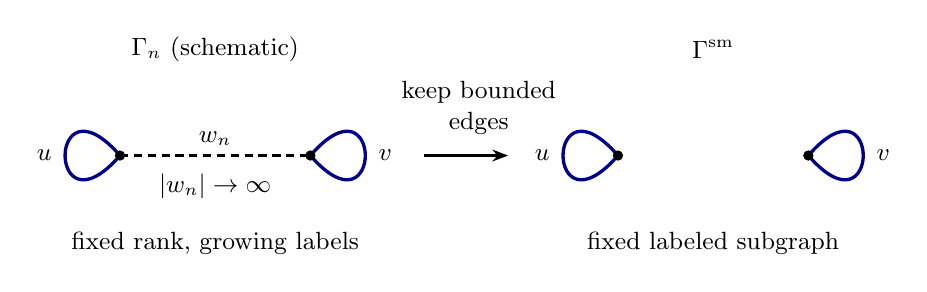
\begin{tikzpicture}[scale=.93, every node/.style={font=\small},
  bounded/.style={draw=blue!55!black,very thick},
  longedge/.style={draw=black,densely dashed,thick}]
\node at (1.3,1.45) {$\Gamma_n$ (schematic)};
\draw[bounded] (0,0) .. controls (-1,1.15) and (-1,-1.15) .. (0,0);
\draw[bounded] (2.6,0) .. controls (3.6,1.15) and (3.6,-1.15) .. (2.6,0);
\draw[longedge] (0,0) -- node[above] {$w_n$}
 node[below=3pt] {$|w_n|\to\infty$} (2.6,0);
\fill (0,0) circle(2pt); \fill (2.6,0) circle(2pt);
\node[left] at (-.8,0) {$u$}; \node[right] at (3.4,0) {$v$};
\draw[-{Stealth[length=2mm]},thick] (4.15,0) -- (5.3,0);
\node[align=center] at (4.9,.65) {keep bounded\\edges};
\node at (8.1,1.45) {$\Gamma^{\mathrm{sm}}$};
\draw[bounded] (6.8,0) .. controls (5.8,1.15) and (5.8,-1.15) .. (6.8,0);
\draw[bounded] (9.4,0) .. controls (10.4,1.15) and (10.4,-1.15) .. (9.4,0);
\fill (6.8,0) circle(2pt); \fill (9.4,0) circle(2pt);
\node[left] at (6,0) {$u$}; \node[right] at (10.2,0) {$v$};
\node at (1.3,-1.2) {fixed rank, growing labels};
\node at (8.1,-1.2) {fixed labeled subgraph};
\end{tikzpicture}
\caption{A fixed natural graph can have arbitrarily long edge labels.
Here the bounded loops survive and the divergent bridge is deleted,
while both natural vertices remain. The small components in this
schematic example are cyclic; a noncyclic small component is not
assumed to exist.}
\label{car:small-figure}
\end{figure}

Each connected component $D$ of $\Gamma^{\mathrm{sm}}$, with a
chosen vertex, gives the subgroup of $P$ consisting of labels of
its based loops.  The map to $R$ is an immersion, so this subgroup
is isomorphic to $\pi_1D$.  Changing the vertex changes its
conjugacy class only.  Components of rank zero or one are allowed.
A bi-infinite reduced path entirely in $D$ lies in its unbased core,
and its labels have endpoints in a translate of the corresponding
subgroup limit set.

\subsection{A finite cofinal family of subgroups}

Let $\mathcal C$ be the set of $P$-conjugacy classes of finitely
generated noncyclic subgroups $Q\le P$ fixing a positively traversed
bilateral path through $e$ pointwise.  Such a path is unique: otherwise its
two finite windows would eventually diverge, contrary to
Proposition~\ref{stat:windows}.  Define
\[
 [Q]\preceq[M]
 \quad\Longleftrightarrow\quad
 Q\le aMa^{-1}\text{ for some }a\in P.
\]
We first verify that this really is a partial order, rather than
merely a preorder.

\begin{lemma}
\label{car:conjugate-containment}
A nontrivial finitely generated subgroup of a finite-rank free group
cannot be properly contained in a conjugate of itself.  Consequently
$\preceq$ is a partial order on $\mathcal C$.
\end{lemma}

\begin{proof}
Suppose $a^{-1}Ma\lneq M$.  No positive power $a^k$ belongs to $M$:
otherwise the nested inclusions
\[
 M\supseteq a^{-1}Ma\supseteq\cdots
 \supseteq a^{-k}Ma^k=M
\]
force equality at every stage.  Thus the Schreier vertices
$Ma^{-n}$, $n\ge0$, are distinct.  Fix a nontrivial reduced word
$w\in M$, of length $L$.  At each of those vertices the word $w$
labels a closed reduced path, since $a^{-n}wa^n\in M$.

The Schreier graph consists of its finite unbased core with trees
attached.  A closed reduced path of length $L$ has its starting
vertex at distance at most $L/2$ from the core: outside it, the
path must travel to the core and return along the same tree
attachment.  The $L/2$-neighborhood of the finite core has only
finitely many vertices.  It cannot contain all the distinct
$Ma^{-n}$, proving the first assertion.  The reverse direction of
conjugate containment follows by replacing $a$ by $a^{-1}$.

If $[Q]\preceq[M]\preceq[Q]$, suitable representatives give
\[
 Q\le aMa^{-1}\le abQ(ab)^{-1}.
\]
The inclusion between the first and last groups is equality by the
first assertion.  Both intermediate inclusions are therefore
equalities, and $[Q]=[M]$.  Reflexivity and transitivity are immediate.
\end{proof}

The following elementary graph bound supplies the compactness step.
It is important here that a core can have bridges.

\begin{lemma}[Bounded circuits in a core]
\label{car:circuits}
Let $C$ be a finite connected graph with no degree-one vertices and
with at least one edge.  Every edge of $C$ lies on an immersed circuit
of length at most $2|E(C)|$, where edges have length one and
$|E(C)|$ counts unoriented edges.
\end{lemma}

\begin{proof}
A nonbridge edge lies on a simple cycle of length at most $|E(C)|$.
If $a$ is a bridge, removing its interior leaves two components,
each containing a cycle.  Indeed, a component without cycles would
be a finite tree with at most one possible vertex of degree one,
which is impossible.  On each side choose a shortest path from
the endpoint of $a$ to a simple cycle, traverse the cycle, and
return along that path.  The resulting based path is reduced and
has length at most twice the number of edges on that side.
Combine these two paths with $a$ and $a^{-1}$.  The joins are
reduced, including the cyclic join, because the based paths remain
on their respective sides of $a$.  The resulting immersed circuit
contains $a$ and has length at most $2|E(C)|$.
\end{proof}

\begin{proposition}[Finite cofinal carriers]
\label{car:finite-carriers}
The noncyclic component subgroup classes of
$\Gamma^{\mathrm{sm}}$ belong to $\mathcal C$ and form a finite
cofinal subset: every $[Q]\in\mathcal C$ is contained, up to
$P$-conjugacy, in one of them.  In particular $\mathcal C$ has only
finitely many maximal elements, and they are exactly the maximal
members of this finite family.
\end{proposition}

\begin{proof}
Let $M$ be a noncyclic subgroup given by loops at a chosen vertex
of a small component.  These same loop labels occur at the
corresponding state of every selected $\Gamma_n$.  By the state
interpretation in Lemma~\ref{car:window-cores}, $M$ fixes an actual
centered window of radius $n$.  The windows obtained for different
$n$ have identical restrictions to any common shape, because
$M$ is noncyclic.  Their compatible restrictions form a bilateral
positive path fixed by $M$.  Thus $[M]\in\mathcal C$.

Now take $[Q]\in\mathcal C$, and let $C(Q)$ be its fixed unbased
core.  Put
\[
 D_Q=2|E(C(Q))|.
\]
For every selected $n$, the group $Q$ is contained in the full
stabilizer of its centered radius-$n$ window.  After translating to
one of our representatives, this inclusion gives a label-preserving
immersion
\[
 C(Q)\longrightarrow\Gamma_n.
\]
One way to see the map directly is to include the minimal
$Q$-invariant subtree in the minimal subtree of the containing
group and take quotients.  Conjugating the containing group merely
translates its subtree and does not change labels.

Choose $n$ so large that every divergent natural edge of
$\Gamma_n$ has length greater than $D_Q$.  Suppose the image of
some edge of $C(Q)$ meets the interior of one of those natural edges.  By
Lemma~\ref{car:circuits}, that source edge lies on an immersed
circuit of length at most $D_Q$.  Its image remains immersed.
At the degree-two interior of a natural edge there is no reduced
way to turn around, so the image circuit traverses that entire
natural edge.  This remains true if its chosen starting point is
in the interior: view the traversal cyclically.  Its length is
then greater than $D_Q$, a contradiction.

The whole image of $C(Q)$ therefore lies in
$\Gamma^{\mathrm{sm}}$.  Since it is connected, it lies in one
small component, with subgroup $M$.  The induced inclusion gives
$[Q]\preceq[M]$, and $M$ is noncyclic because it contains a
noncyclic subgroup.  Notice that no compatible choices of
conjugating elements were required as $n$ varied: once all long
edges exceed $D_Q$, the argument applies to every possible
label-preserving immersion.

There are finitely many small components.  A maximal member of
their noncyclic subgroup classes is maximal in all of
$\mathcal C$: any larger class lies below another member of the
finite family and hence would contradict its maximality there.
Conversely a maximal class in $\mathcal C$ equals a small class
above it.  This proves the final assertion.
\end{proof}

We have now replaced the possibly unbounded window cores by a
finite set of maximal subgroup carriers.  The next step uses
maximality to make a return transfer surjective.  If there are no
noncyclic small components, $\mathcal C$ is empty and all statements
about its maximal members below are vacuous.

\subsection{Return automorphisms}

Moving one edge forward along the path fixed by $Q$ and expressing
$Q$ in the new edge coordinates defines a map
\[
 F:\mathcal C\longrightarrow\mathcal C.
\]
This moves subgroup coordinates, not individual support lines;
it is defined for every class in $\mathcal C$.

\begin{proposition}[Atoroidal return]
\label{car:return}
The map $F$ is an order-preserving bijection with order-preserving
inverse.  It permutes the finite set of maximal classes of
$\mathcal C$.  For every representative $M$ of such a class, there
are an integer $p\ge1$ and an element $v\in G$ of height $p$ such
that
\[
 v^{-1}Mv=M.
\]
The automorphism $\alpha:M\to M$, $\alpha(m)=v^{-1}mv$, is
atoroidal: no nontrivial conjugacy class in $M$ is periodic under
$\alpha$.
\end{proposition}

\begin{proof}
Choose a frame $h$ for the next edge on the unique path fixed by
$Q$.  Transfer gives $h^{-1}Qh\le P$.  Another frame has the form
$hq$, $q\in P$, and conjugates this output inside $P$.
Conjugating $Q$ inside $P$ translates its path and gives the same
output class.  Thus $F$ is well defined.  Moving backward is its
inverse.  If $Q\le M$ after choosing representatives, both groups
fix the same path by noncyclic uniqueness; the same partial
conjugation preserves their inclusion.  This proves the order
assertions.

An order automorphism permutes maximal elements.  There are
finitely many of them by Proposition~\ref{car:finite-carriers},
so $F^p[M]=[M]$ for some $p\ge1$.  If their number is $N$, one
may choose $p\le N$.  Let $h$ be a frame for the $p$th forward
edge.  There exists $c\in P$ with
\[
 h^{-1}Mh=cMc^{-1}.
\]
Set $v=hc$.  Then $v$ has height $p$ and
$v^{-1}Mv=M$, which proves that the return map is an onto
automorphism.

Suppose $\alpha^k(w)=u^{-1}wu$ for some nontrivial $w\in M$,
$u\in M$, and $k\ge1$.  Then
\[
 g=v^ku^{-1}
\]
commutes with $w$.  Its height is $kp\ne0$, whereas $w$ has
height zero and infinite order.  A relation $w^a g^b=1$ forces
$b=0$ by height, then $a=0$.  Thus
$\langle w,g\rangle\cong\mathbb Z^2=BS(1,1)$, contrary to
BS-freeness.  This proves atoroidality without using hyperbolicity
of $G$ or the flaring statement under investigation.
\end{proof}

The element $v$ preserves the bilateral path fixed by $M$:
normalizing $M$ sends that path to another path fixed by $M$.
Both paths contain $ve$, so uniqueness in that edge's coordinates
identifies them.  It translates the path forward by $p$
edges.  In particular, the paths from $e$ to $v^be$ and to
$v^{-b}e$ are the concatenated positive and negative return
paths, respectively, and are reduced.

\subsection{Expansion and vanishing carrier mass}

For an element $w$ of a finitely generated free group with a chosen
basis, write $|w|$ for based word length and $\ell(w)$ for cyclic
length.  Brinkmann's theorem states that an automorphism $\alpha$
of a finite-rank free group with no nontrivial periodic conjugacy
class is hyperbolic: there exist $b_0\ge1$ and $\lambda_0>1$ such
that
\[
 \lambda_0|w|
 \le\max\{|\alpha^{b_0}(w)|,|\alpha^{-b_0}(w)|\}
 \quad\text{for every }w
\]
\cite[Theorem~1.1 and the definition of a hyperbolic
automorphism]{Brinkmann2000HyperbolicAutomorphisms}.  These are based lengths in a fixed
free basis.  We need both a stronger expansion factor and a
consequence for arbitrary currents; the latter uses a sum, not
a maximum.

\begin{lemma}[Expansion on elements and currents]
\label{car:expansion}
Let $M,v,\alpha$ be as in Proposition~\ref{car:return}, and choose
a free basis of $M$.  There exist $b\ge1$, an automorphism
$\beta=\alpha^b$, and $\lambda>4$ such that
\begin{align}
 \lambda|w|_M
 &\le\max\{|\beta(w)|_M,|\beta^{-1}(w)|_M\},
 &&w\in M,                                      \label{car:based}\\
 \lambda\ell_M(w)
 &\le\max\{\ell_M(\beta(w)),\ell_M(\beta^{-1}(w))\},
 &&w\in M.                                      \label{car:cyclic}
\end{align}
For every $M$-current $\sigma$ one has
\begin{equation}
 \lambda\|\sigma\|_M
 \le\|\beta_*\sigma\|_M+
       \|(\beta^{-1})_*\sigma\|_M.
 \label{car:current}
\end{equation}

The partial conjugations along the paths to $v^be$ and $v^{-b}e$
have domains
\[
 S_+=P\cap v^bPv^{-b},\qquad
 S_-=P\cap v^{-b}Pv^b,
\]
respectively.  These are finitely generated full window stabilizers,
and both contain $M$.  Their boundary transfers are defined on all
of $\partial^2\Lambda S_+$ and $\partial^2\Lambda S_-$.
The transfers $\Theta_+,\Theta_-$ restrict on $\partial^2\Lambda M$ to
$\beta,\beta^{-1}$, respectively, and preserve $\mu$ on their
irrational-endpoint domains.
\end{lemma}

\begin{proof}
Apply Brinkmann's theorem to $\alpha$, and put
$\gamma=\alpha^{b_0}$.  If
$|\gamma(w)|_M\ge\lambda_0|w|_M$, applying the inequality to
$\gamma(w)$ shows that its expanding direction must again be
forward: its backward image has length $|w|_M$, which is strictly
less than $\lambda_0|\gamma(w)|_M$ for $w\ne1$.  Induction gives
\[
 |\gamma^k(w)|_M\ge\lambda_0^k|w|_M.
\]
The analogous statement holds for a backward initial expanding
direction.  Choose $k\ge1$ with $\lambda_0^k>4$, and set
$b=b_0k$, $\beta=\alpha^b$, and $\lambda=\lambda_0^k$.
This proves~\eqref{car:based}; it also holds for $w=1$.
Apply it to $w^q$, divide by $q$, and let $q\to\infty$.
The identity $\lim_{q\to\infty}|w^q|_M/q=\ell_M(w)$ proves
\eqref{car:cyclic}.

For a counting current $\eta_w$, the cyclic inequality and
$\|\eta_w\|_M=\ell_M(w)$ imply~\eqref{car:current}, with the
maximum replaced by the sum.  The sum form is linear and therefore
holds for all finite nonnegative linear combinations of counting
currents.  We give the approximation argument extending it to
every current.

Fix $k\ge2$.  The directed graph with vertices the reduced words
of length $k-1$ and edges the reduced words of length $k$ has an
edge from a word's prefix to its suffix.  The masses
$\langle u,\sigma\rangle$ of directed segment cylinders based at the
identity and labeled by length-$k$ words $u$ form a
nonnegative circulation: both incoming and outgoing sums at a
vertex equal its length-$(k-1)$ cylinder mass.  Any such circulation
is a finite nonnegative sum of directed cycle circulations.
Indeed, follow positive-flow edges to find a directed cycle,
subtract the minimum edge flow on that cycle, and repeat; at
least one positive edge disappears at each step.

Write the circulation as $\sum_i a_i C_i$.  Each directed cycle
is the block circulation of a cyclically reduced word $w_i$,
including multiplicities if that word is a proper power.  Let
$C_i^{\mathrm{flip}}$ be the circulation obtained by reversing
words and inverting letters.  The counting current $\eta_{w_i}$
has circulation $C_i+C_i^{\mathrm{flip}}$.  Since $\sigma$ is
flip-invariant, the current
\[
 \sigma_k=\frac12\sum_i a_i\eta_{w_i}
\]
has exactly the same masses as $\sigma$ on all length-$k$
cylinders.  Summing over extensions gives equality on all shorter
word cylinders as well.  This also covers graph loops and
period-one words; proper powers have their prescribed counting
multiplicities.

As $k\to\infty$, the currents $\sigma_k$ converge to $\sigma$
on every cylinder, hence in the current topology.  Their norms
are equal to that of $\sigma$, since length-one masses already
agree.  Continuity of the norm and of the current maps induced
by $\beta^{\pm1}$ now proves~\eqref{car:current}.

Finally, the return paths are reduced as observed after
Proposition~\ref{car:return}.  Fixing their first and last edges
is equivalent to fixing the intervening segment, so their full
stabilizers in $P$ are exactly $S_+$ and $S_-$ above.  Since
$v$ normalizes $M$, both contain $M$.  Their partial conjugations
are $x\mapsto v^{-b}xv^b$ and $x\mapsto v^bxv^{-b}$, whose
restrictions are $\beta$ and $\beta^{-1}$.  The boundary and
measure assertions follow from Proposition~\ref{stat:windows}.
\end{proof}

\begin{proposition}[Zero mass on a maximal carrier]
\label{car:zero-mass}
For every maximal carrier $M$ supplied by
Proposition~\ref{car:finite-carriers},
\[
 \mu(\partial^2\Lambda M)=0.
\]
The same holds for every $P$-translate of this line set.
\end{proposition}

\begin{proof}
Use the boundary embedding of $M$ in $P$ to pull back the
restriction of $\mu$ to the relatively closed subset
$\partial^2\Lambda M$ of $\partial^2P$.  This gives an
$M$-current $\sigma$: invariance and flip-invariance come from
$\mu$, and the restriction is Radon because the boundary
embedding sends compact subsets of $\partial^2M$ to compact
subsets of $\partial^2P$.

Both endpoints are irrational outside a $\mu$-null set by
Proposition~\ref{stat:transfers}.  On those lines the return transfer
$\Theta_+$ is measure-preserving, maps
$\partial^2\Lambda M$ onto itself, and agrees with $\beta$.
Thus $\beta_*\sigma=\sigma$; the inverse has the same property.
Equation~\eqref{car:current} gives
\[
 \lambda\|\sigma\|_M\le2\|\sigma\|_M.
\]
Since $\lambda>4$, this forces $\sigma=0$.  Hence the restricted
measure is zero.  Translation invariance of $\mu$ gives the
last assertion.
\end{proof}

This is a measure conclusion, not a support conclusion: a closed
set of measure zero can still contain lines of $\Omega$.  The
next section uses the return expansion to exclude precisely those
possible support lines.

\section{Expansion and periodic lines in the support}
\label{exp:section}

We retain the nonzero stationary current $\mu$, its closed support
$\Omega\subset\partial^2P$, and the invariant conull set $\mathcal U$
from the preceding sections. Our purpose here is to exclude periodic
lines from $\Omega$. This is stronger than atomlessness: a line can belong
to the support while having measure zero. Only after proving this stronger
assertion will we extend the trajectory construction from $\mathcal U$
to every line of $\Omega$.

The obstruction is a possible carrier line in the support despite its
zero measure. We will expand a positive-measure cylinder near such a
line along a fixed return. If the whole cylinder follows the return
forever, its translated images concentrate on the zero-mass carrier
set. If a line leaves the prescribed return domain, it follows a
competing window; the cyclic intersection of the two window stabilizers
forces a periodic middle in their long common segment. Lemma~\ref{exp:finite-failure}
records this alternative quantitatively. We first use it to produce
periodic support from carrier support, then use whole-period pullback
to rule out periodic support itself.

The window results provide the finite data for this argument. For each
fixed shape there are finitely many representative cores of noncyclic
window stabilizers; only finitely many actual windows have their hulls
meeting a fixed ball. Distinct actual windows of that shape have at
most cyclic common stabilizer, and an irrational endpoint determines
at most one window (Proposition~\ref{stat:windows} and
Lemma~\ref{stat:window-finiteness}). We will also use the fixed small
subgraph of the selected cores $\Gamma_n$ from
Definition~\ref{car:small-graph}.

Let $M\le P$ represent one of the maximal noncyclic carrier classes.
Proposition~\ref{car:return} and Lemma~\ref{car:expansion} supply
an automorphism $\beta$ of $M$, a number $\lambda>4$, and fixed forward
and backward window transfers $\Theta_+$ and $\Theta_-$ with domains
\[
 \partial^2\Lambda S_+\quad\hbox{and}\quad
 \partial^2\Lambda S_-,\qquad M\le S_+,S_-\le P.
\]
Here and below $\partial^2\Lambda K$ denotes the ordered pairs of
distinct points of the limit set of $K$. On the boundary of $M$ these
transfers are respectively $\beta$ and $\beta^{-1}$. They are induced
by the actual paths to the positive and negative powers of the return
frame. In an $M$-basis,
\begin{equation}
 \lambda |w|_M\le
 \max\{|\beta(w)|_M,|\beta^{-1}(w)|_M\}
 \qquad(w\in M).
 \label{exp:based-inequality}
\end{equation}
The same inequality holds for cyclic lengths. Moreover,
Proposition~\ref{car:zero-mass} gives
\begin{equation}
 \mu(\partial^2\Lambda M)=0.
 \label{exp:zero-carrier-mass}
\end{equation}
All transfers preserve $\mu$ on their domains in $\mathcal U$ and
take those domains into $\mathcal U$. No assertion about their action
on arbitrary support lines is being assumed.

We call a line of the $P$-Cayley tree an \emph{$M$-line} if its two
endpoints belong to $\Lambda M$. It corresponds to a unique line of
the $M$-Cayley tree under the boundary embedding. A periodic line is
the axis of a nontrivial element. Its primitive translation is a
generator of its cyclic stabilizer; this does not mean a member of a
free basis. When both $M$ and $P$ occur, we specify in which group the
translation is primitive.

\subsection{Uniform geometric estimates}

Write $\mathcal C_Q$ for the unit-edge Cayley tree of a finitely
generated free group $Q$ with a fixed basis. A homomorphism on vertices
is extended over each edge by its reduced image path. The image of a
geodesic under a fixed injective homomorphism is a uniform
quasigeodesic; its tightened line is at uniformly bounded Hausdorff
distance from it. We first record the consequence needed both here and
in the final argument.

\begin{lemma}[Nearness and order under a fixed transfer]
\label{exp:transport}
Let $a:Q\to F$ and $b:Q\to F'$ be injective homomorphisms between
finitely generated free groups with fixed bases. For every $D\ge0$
there are constants $E,T\ge0$ with the following properties.
Let $L$ be an oriented line of $\mathcal C_Q$, and let $L_a,L_b$
be its tightened image lines in $\mathcal C_F,\mathcal C_{F'}$.
If $q\in Q$ satisfies $d(a(q),L_a)\le D$, then
\[
 d(b(q),L_b)\le E.
\]
If two such elements $q_1,q_2$ have projections to $L_a$ positively
ordered and separated by more than $T$, then their projections to
$L_b$ are in the same order. As their separation on $L_a$ tends to
infinity, their separation on $L_b$ tends to infinity, uniformly over
all $L,q_1,q_2$.
\end{lemma}

\begin{proof}
Fix Hausdorff bounds between each tightened image line and the images
of vertices of $L$. Choose a vertex $u\in L$ whose $a$-image is
uniformly close to a point of $L_a$ closest to $a(q)$. The lower
quasi-isometry bound for $a$ gives a bound on $d_Q(q,u)$ depending
only on $D$ and $a$. The upper bound for $b$, followed by its
line Hausdorff bound, proves the first assertion.

For the order assertion, first consider actual vertices $u<v$ on an
oriented source line and one fixed embedding $f$. The image of $v$ is
within a fixed distance of the geodesic from $f(u)$ to $f(z)$ for every
source vertex $z$ sufficiently far beyond $v$. Projecting to the
tightened image line and letting $z$ tend to its positive end shows
that the projection of $f(v)$ cannot lie more than a fixed distance
behind that of $f(u)$. On the other hand, the distance between these
projections is at least
\[
 c_f d_Q(u,v)-C_f
\]
for fixed $c_f>0,C_f\ge0$, by the lower embedding bound and the
line Hausdorff bound. Thus sufficiently separated vertices have
projections in the correct order, with separation tending to infinity.

Apply this first to $a$ and then to $b$. Replace $q_i$ by vertices
$u_i\in L$ at the uniformly bounded distance obtained in the first
paragraph. Their image projections change by uniformly bounded
amounts. Sufficient positive separation of the $a(q_i)$ therefore
forces $u_1<u_2$ with large separation, and then forces the asserted
order and separation of the $b(q_i)$. All constants came from the
fixed embeddings and $D$.
\end{proof}

We will also use two elementary properties of trees. If $x,y$ lie
within $D$ of a geodesic line $L$, the part of $[x,y]$ farther than
$D$ from both endpoints lies on $L$. Indeed, project $x,y$ to $L$;
if the projections are distinct, the connecting segment enters and
leaves $L$ there. If they coincide, then $d(x,y)\le2D$, so there
is no point farther than $D$ from both endpoints.
The same assertion holds for an arbitrary convex subtree. Secondly,
the lines meeting a fixed finite ball form a compact subset of line
space: they are a finite union of the compact sets of lines through
its vertices. A current has finite mass on this set.

\begin{lemma}[Expansion with fixed trimming]
\label{exp:trimming}
Fix a maximal carrier $M$ and the maps above. There are constants
$Q\ge0$ and $L_*>0$ with the following property. Let $L$ be an
oriented $M$-Cayley-tree line, let $x,y$ be vertices on $L$ with
$d_M(x,y)=l\ge L_*$, and let $\mathcal A\subset\mathcal U$ be
a Borel set whose lines lie within $Q$ of both $x,y$ in
$\mathcal C_P$. Suppose a sign $\epsilon\in\{+1,-1\}$ satisfies
\[
 d_M(\beta^\epsilon x,\beta^\epsilon y)\ge\lambda l.
\]
If every line of $\mathcal A$ belongs to
$\partial^2\Lambda S_\epsilon$, then its image
$\mathcal A'=\Theta_\epsilon(\mathcal A)$ has the same measure,
lies in $\mathcal U$, and admits vertices $x',y'$ on the tightened
line $\beta^\epsilon L$ such that
\[
 d_P(x',\ell),d_P(y',\ell)\le Q\quad(\ell\in\mathcal A'),
 \qquad d_M(x',y')\ge2l.
\]
The same sign satisfies
\[
 d_M(\beta^\epsilon x',\beta^\epsilon y')
 \ge\lambda d_M(x',y').
\]
The constants are independent of $L,x,y,\mathcal A$ and of the
number of times this assertion is applied.
\end{lemma}

\begin{proof}
Choose $Q$ bounding the distance of every $M$-vertex on a geodesic
segment or line to its tightened $P$-image, and bounding the reverse
distance from that image to images of vertices. Increase it if
necessary. Applying Lemma~\ref{exp:transport} to the two fixed
window maps gives a common $C_1$ such that
$u=\beta^\epsilon x$ and $z=\beta^\epsilon y$ are within $C_1$
of every line in $\mathcal A'$.

Choose lower embedding constants $a>0,b\ge0$ with
\[
 d_P(g,h)\ge a d_M(g,h)-b\qquad(g,h\in M).
\]
Let $B$ be a common vertex-to-line bound for the two automorphisms
$\beta^{\pm1}$ of $M$. Choose an integer $R$ such that
\begin{equation}
 R>B,\qquad aR-b-Q>C_1.
 \label{exp:R-choice}
\end{equation}
Delete $R$ edges at both ends of $[u,z]$ in $\mathcal C_M$, and
call its new endpoints $x',y'$. The first inequality in
\eqref{exp:R-choice} puts them on the tightened line
$\beta^\epsilon L$. Their $P$-images lie within $Q$ of
$[u,z]_P$. If $v$ is either new endpoint, its projection to this
segment has distance at least $aR-b-Q>C_1$ from each end.
The intervening part of $[u,z]_P$ lies on every line of
$\mathcal A'$, by the tree observation. Hence $x',y'$ are still
within $Q$ of every such line.

Put
\[
 K=\max\{\operatorname{Lip}(\beta),
                 \operatorname{Lip}(\beta^{-1})\}.
\]
The new length $l'$ satisfies
\begin{equation}
 l'\ge\lambda l-2R,
 \qquad
 d_M(\beta^{-\epsilon}x',\beta^{-\epsilon}y')
 \le l+2KR.
 \label{exp:trim-estimates}
\end{equation}
Choose $L_*$ sufficiently large that, for every $l\ge L_*$,
\[
 \lambda l-2R\ge2l,
 \qquad l+2KR<2\lambda l.
\]
Then the opposite direction at the new pair has length strictly
less than $\lambda l'$. Inequality~\eqref{exp:based-inequality}
forces expansion in the original direction. Measure preservation
and membership in $\mathcal U$ follow from the invariant conull
transfer construction. Since the maps are fixed boundary
homeomorphisms on their domains, the image set is Borel.
\end{proof}

\subsection{A failed return produces a periodic segment}

Fix the carrier $M$, its return maps, and the constants in
Lemma~\ref{exp:trimming}. The next lemma supplies the common construction
for both support arguments. Its reference line is transferred in the
boundary of $M$; only the competing line in its conclusion is asserted
to lie in $\Omega$.

\begin{lemma}[Finite failure of an expanding return]
\label{exp:finite-failure}
There are constants $L_0\ge L_*$, $c>0$, $C_2\ge0$, and an integer
$D\ge1$, depending only on the fixed splitting, carrier, and return maps, with
the following property. Let $\eta\in\Omega\cap\partial^2\Lambda M$,
let $L$ be its corresponding oriented $M$-Cayley-tree line, and choose
vertices $x_0<y_0$ on $L$ with $l_0=d_M(x_0,y_0)\ge L_0$. Suppose
$\epsilon\in\{+1,-1\}$ satisfies
\[
 d_M(\beta^\epsilon x_0,\beta^\epsilon y_0)\ge\lambda l_0.
\]
Then there are $n\ge0$, a line $\ell\in\mathcal U$, and an oriented
periodic $P$-line $\zeta$ of primitive period at most $D$ such that
$\ell$, $\zeta$, and the tightened $P$-image $\eta_n$ of
$\beta^{\epsilon n}L$ share a segment of length at least
\begin{equation}
 c\,2^n l_0-C_2.
 \label{exp:failure-overlap}
\end{equation}
The endpoints of $\zeta$ lie in the limit sets of the stabilizers of
two distinct actual windows of the shape defining $\Theta_\epsilon$.
One is the prescribed window, with stabilizer $S_\epsilon$.
\end{lemma}

\begin{proof}
Choose $L_0\ge L_*$ large enough that the projections of $x_0,y_0$
to $\eta$ are distinct and occur in that order. This choice is uniform
by Lemma~\ref{exp:transport}; we will increase $L_0$ once more below.
The cylinder prescribing the directed segment between those projections
has positive finite measure, since $\eta\in\Omega$. Its intersection
with $\mathcal U$ is a Borel set $\mathcal A_0$ of positive finite
measure, every line of which is within $Q$ of $x_0,y_0$.

Attempt to apply $\Theta_\epsilon$ successively to the entire
current set. At time $n$, call the attempt a \emph{failure} if
$\mathcal A_n$ is not contained in
$\partial^2\Lambda S_\epsilon$. Otherwise define
$\mathcal A_{n+1}=\Theta_\epsilon(\mathcal A_n)$ and use
Lemma~\ref{exp:trimming} to obtain the next segment. As long as
the process continues, its vertices $x_n,y_n$ lie on
$\beta^{\epsilon n}L$, their distance $l_n$ is at least
$2^n l_0$, and every line of $\mathcal A_n$ lies within $Q$ of
both vertices. Its measure is the fixed number
$\delta=\mu(\mathcal A_0)>0$.

\smallskip\noindent
\emph{The process cannot continue forever.}
Choose an $M$-vertex $a_n$ within one edge of the midpoint of
$[x_n,y_n]_M$ and
translate $\mathcal A_n$ by $a_n^{-1}$. The central portion of
$[x_n,y_n]_P$ belongs to every line of $\mathcal A_n$.
The image of $a_n$ is uniformly close to this segment, and the
lower embedding bound puts its projection arbitrarily far from
both endpoints as $n$ increases. That projection therefore lies
in the common central portion. Thus the translated sets
eventually lie in one compact set $\mathcal K$ of lines meeting a
fixed ball. Their measures are still $\delta$.

Every subsequential limit of these lines belongs to
$\partial^2\Lambda M$. To see this, take a subsequence of the
centered $M$-segments. Both halves tend to infinite length, so a
further subsequence converges to a bi-infinite $M$-geodesic. Its
quasigeodesic image in $P$ has two distinct boundary endpoints,
and its tightened line is the limit of the growing common central
segments. These endpoints lie in $\Lambda M$.

Consequently every relative neighborhood of
$\mathcal K\cap\partial^2\Lambda M$ in $\mathcal K$ contains
all sufficiently late translated sets. Otherwise points outside
one such neighborhood would have a contrary subsequential limit
in the compact set $\mathcal K$. Outer regularity of the finite
measure on $\mathcal K$ now gives
\[
 \mu(\mathcal K\cap\partial^2\Lambda M)\ge\delta,
\]
contrary to \eqref{exp:zero-carrier-mass}.

\smallskip\noindent
\emph{A failure produces a bounded-period axis.}
Suppose failure occurs at time $n$, and choose
$\ell\in\mathcal A_n\setminus\partial^2\Lambda S_\epsilon$.
This line has an actual trajectory for the same finite one-sided
window. Its stabilizer $K$ is noncyclic, and this actual path differs
from the prescribed path: equality would put both endpoints of
$\ell$ in $\Lambda S_\epsilon$.

Both $\ell$ and the tightened image $\eta_n$ of
$\beta^{\epsilon n}L$ pass within $Q$ of $x_n,y_n$. Since
$x_n,y_n\in M\le S_\epsilon$, their distances from
$\operatorname{Hull}(\Lambda S_\epsilon)$ equal the fixed number
$d_P(1,\operatorname{Hull}(\Lambda S_\epsilon))$. Set
\[
 H_\epsilon=\max\{Q,
             d_P(1,\operatorname{Hull}(\Lambda S_\epsilon))\}.
\]
Deleting $H_\epsilon$ from both ends of $[x_n,y_n]_P$ leaves a
segment in $\ell$, in $\eta_n$, and in the prescribed stabilizer
hull. It also lies in $\operatorname{Hull}(\Lambda K)$ because
$\ell$ does. Its length is at least
\begin{equation}
 a l_n-C,
 \label{exp:central-overlap}
\end{equation}
where $a>0,C\ge0$ depend only on the fixed maps and embeddings.
In particular, no constant from the varying competing subgroup $K$
is needed.

Read this segment in the two finite stabilizer cores. Their fiber
product pairs core states, with an edge for each pair of equally
labeled edges. At an actual vertex $z$ the corresponding pair of states represents the two
paths translated by $z^{-1}$. They remain distinct. Every loop in
the corresponding component of the fiber product therefore fixes
both paths, so its fundamental group injects into an at-most-cyclic
group, by Proposition~\ref{stat:windows}. The component has rank at most
one. Since the window is fixed, there are only finitely many core
representatives, and the numbers of unoriented edges in all relevant fiber products
are bounded by one integer $D\ge1$. Conjugating a stabilizer preserves its labeled
unbased core and changes only the state used for this reading.

Increase $L_0$ so that $aL_0-C>2D+1$, taking the maximum of
the constants for the two signs. This ensures that every failure
reading is long enough to contain a circuit. A reduced path in a
finite tree has length at most its number of edges. A connected
rank-one finite graph consists of one circuit with trees attached,
so a sufficiently long reduced path follows that circuit between
initial and terminal pieces of length at most $D$.
Our reading therefore has a central periodic portion of length at
least $a l_n-C-2D$. Extend it in the absolute Cayley tree to an
oriented periodic line $\zeta$. Its primitive $P$-period is at most
$D$. Unfolding the circuit in each core puts its endpoints in both
actual window stabilizer limit sets. Since $l_n\ge2^n l_0$, this
proves \eqref{exp:failure-overlap}, with constants enlarged uniformly
over the two signs. The line $\ell$ belongs to $\mathcal U$, as
required.
\end{proof}

The failure need not occur on a set of positive measure. Its chosen
line already belongs to $\mathcal U\subset\Omega$, which is enough
for the support limit below. Positive mass rules out indefinite
transfer of the whole cylinder. Figure~\ref{exp:failure-figure}
shows how the two actual windows produce the periodic middle.

\begin{figure}[ht]
\centering
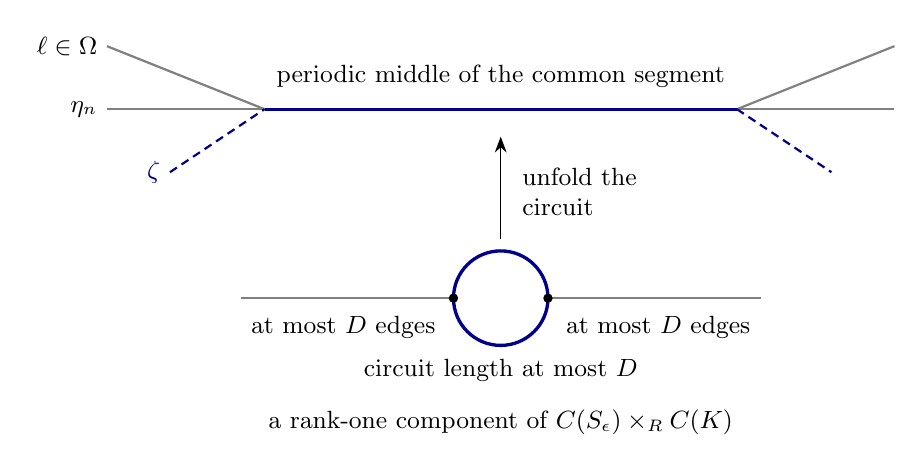
\begin{tikzpicture}[every node/.style={font=\small}]
\draw[gray,thick] (0,2.4) -- (10,2.4);
\draw[gray,thick] (0,3.2) -- (2,2.4);
\draw[gray,thick] (8,2.4) -- (10,3.2);
\draw[blue!55!black,very thick] (2,2.4) -- (8,2.4);
\draw[blue!55!black,densely dashed,thick] (.8,1.6) -- (2,2.4);
\draw[blue!55!black,densely dashed,thick] (8,2.4) -- (9.2,1.6);
\node[left] at (0,2.4) {$\eta_n$};
\node[left] at (0,3.2) {$\ell\in\Omega$};
\node[left,blue!55!black] at (.8,1.6) {$\zeta$};
\node[above] at (5,2.55) {periodic middle of the common segment};
\draw[gray,thick] (1.7,0) -- (4.4,0);
\draw[gray,thick] (5.6,0) -- (8.3,0);
\draw[blue!55!black,very thick] (5,0) circle (.6);
\fill (4.4,0) circle (1.7pt);
\fill (5.6,0) circle (1.7pt);
\draw[-{Stealth[length=2mm]},thin] (5,.75) -- (5,2.05);
\node[right,align=left] at (5.15,1.35) {unfold the\\circuit};
\node[below] at (3,-.1) {at most $D$ edges};
\node[below] at (7,-.1) {at most $D$ edges};
\node[below] at (5,-.65) {circuit length at most $D$};
\node[below] at (5,-1.3)
 {a rank-one component of $C(S_\epsilon)\mathbin{\times_R}C(K)$};
\end{tikzpicture}
\caption{At a failed return, $\eta_n$ and a competing support line
$\ell$ share a long segment in two window-stabilizer hulls. Its reading
in the core fiber product lies in a rank-one component, shown below.
The initial and terminal tree portions have bounded length; between
them the reading follows the circuit. Unfolding that circuit gives the
periodic middle and its extension $\zeta$. The figure is schematic;
only $\ell$ is asserted to lie in the support.}
\label{exp:failure-figure}
\end{figure}

\begin{proposition}
\label{exp:carrier-periodic}
If $\Omega$ contains a line carried, up to translation, by a maximal
noncyclic carrier $M$, then $\Omega$ contains a periodic line.
\end{proposition}

\begin{proof}
Translate the given line into $\partial^2\Lambda M$. Choose
successively longer segments on its corresponding $M$-line and,
for each segment, a sign supplied by \eqref{exp:based-inequality}.
Apply Lemma~\ref{exp:finite-failure}, passing to a subsequence with
the same sign. Its support line and bounded-period axis share a
segment whose length tends to infinity.

Recenter this shared segment
by an $M$-translation chosen near its midpoint on $\eta_n$.
The translated periodic axes have period at most $D$ and meet a
fixed ball. There are only finitely many such axes: there are only
finitely many cyclic labels of length at most $D$, and finitely many
ways for one of their axes to meet that ball. Along a subsequence
the periodic axis is fixed. The translated lines $\ell\in\Omega$
agree with it on segments tending to infinity in both directions,
so they converge to it. Closedness of $\Omega$ proves that this
periodic line belongs to $\Omega$.
\end{proof}

\subsection{Pulling back whole periods}

The next lemma controls the number of periods in a common segment.
Controlling only its metric length would be insufficient, since a
period can grow under an inverse automorphism.

\begin{lemma}[Bounded loss of periods]
\label{exp:period-pullback}
Let $\psi$ be an automorphism of a finitely generated free group $M$
with a fixed basis. There is an integer $C_4\ge0$, depending only on
$\psi$, with the following property. Suppose two lines $L_1,L_2$
of $\mathcal C_M$ share a segment $[u,z^k u]$, where $u$ is a
vertex, $z$ translates $L_2$, and $k>C_4$. Their tightened
$\psi$-images share a segment consisting of $k-C_4$ whole
$\psi(z)$-periods. If $z$ is primitive as a translation in $M$,
then so is $\psi(z)$.
\end{lemma}

\begin{proof}
Choose an integer $B\ge0$ such that the image of any vertex on any
line is within $B$ of the tightened image line. Such a uniform
constant exists by the quasigeodesic line bound for the fixed map
$\psi$. Put $q=2B+1$ and $C_4=2q$.

Write $L_i'=\psi L_i$ for the tightened images and $z'=\psi(z)$.
The line $L_2'$ is the axis of $z'$. If $a$ is the projection of
$\psi(u)$ onto this axis, the projection of the other endpoint
image is exactly
\[
 \pi_{L_2'}\bigl(\psi(z^ku)\bigr)
 =\pi_{L_2'}\bigl(z'^k\psi(u)\bigr)=z'^k a,
\]
because projection onto an invariant line commutes with its
translation. Both endpoint images lie within $B$ of both output
lines. Thus $a,z'^ka$ lie within $2B$ of $L_1'$.

The translation length of $z'$ is an integer at least one. The
vertices $z'^q a$ and $z'^{k-q}a$ therefore lie farther than
$2B$ from both ends of $[a,z'^ka]$ and occur in the stated order.
The tree observation puts their joining segment on $L_1'$, and
it already lies on $L_2'$. It has exactly $k-2q=k-C_4$ full
periods, with both endpoints in the same integer $z'$-orbit.
There is no additional phase loss. Automorphisms preserve being a
non-power, proving the final assertion.
\end{proof}

\begin{lemma}[Agreement of periodic labels]
\label{exp:periodic-labels}
Two bi-infinite label sequences with respective positive integer
periods $a,b$ that agree on $a+b$ consecutive positions agree
everywhere. Consequently two oriented periodic lines in a labeled
Cayley tree with such a common segment are the same actual line.
\end{lemma}

\begin{proof}
Number the common positions $0,\ldots,a+b-1$. For
$0\le i<a$, the letter at position $i$ equals the letter at
$i+b$ by the second period. By the first period this equals the
letter at $(i+b)\bmod a$. Thus the first period pattern is
invariant under addition by $b$ modulo $a$, and is periodic with
period $d=\gcd(a,b)$. The first $b$ common letters then show that
the second pattern is the same $d$-periodic pattern. Both entire
sequences therefore agree. A label and an initial vertex determine
a unique path in a Cayley tree, so equality of the sequences and
the shared segment identifies the actual lines.
\end{proof}

\begin{lemma}[A bounded-period axis near a carrier]
\label{exp:carrier-period}
Let $M\le P$ be a finitely generated nontrivial subgroup, with fixed
bases, and fix $D\ge1$. There are constants $L_D,B_D$ such that if
a periodic $P$-line $\zeta$ of primitive period at most $D$ shares
a segment of length at least $L_D$ with an $M$-line, then $\zeta$
is itself an $M$-line. Its primitive translation in $M$ has cyclic
$M$-length at most $B_D$.
\end{lemma}

\begin{proof}
Let $V$ be the number of vertices in the finite core of $M$ in the
$P$-rose, and take $L_D=(V+1)D$. The common segment lies in
$\operatorname{Hull}(\Lambda M)$. If $r$ is the actual primitive
$P$-translation of $\zeta$, that segment contains $V+1$ successive
vertices $r^i z_0$ in one period phase. Two have the same core state:
\[
 M r^i z_0=M r^j z_0\qquad(0\le i<j\le V).
\]
Cancelling $z_0$ gives $r^{j-i}\in M$. Thus a power of the
translation of this very axis belongs to $M$, and the whole line
has endpoints in $\Lambda M$.

If $z$ is its primitive translation in $M$, it is the smallest
positive power of $r$ belonging to $M$, up to orientation. Hence
$z=r^q$ for some $1\le q\le V$. Choose embedding constants with
\[
 |g|_M\le A|g|_P+B\qquad(g\in M).
\]
Apply this to powers of $z$, divide by the exponent, and take the
limit to obtain
\begin{equation}
 \ell_M(z)\le A\ell_P(z)\le AVD.
 \label{exp:carrier-period-bound}
\end{equation}
Thus $B_D=AVD$ suffices. The two primitive translations need not
coincide, which is why both groups are specified.
\end{proof}

\subsection{Exclusion of periodic support lines}

\begin{proposition}
\label{exp:no-periodic}
The support $\Omega$ contains no periodic line.
\end{proposition}

\begin{proof}
Suppose $\eta_0\in\Omega$ is periodic.

\smallskip\noindent
\emph{Step 1: construct a trajectory and locate a maximal carrier.}
We first construct one compatible trajectory for $\eta_0$; uniqueness
at its rational endpoints is not assumed.

Approximate $\eta_0$ by lines of $\mathcal U$. For each fixed
centered window, their stabilizer hulls meet a common finite ball.
Lemma~\ref{stat:window-finiteness} lets us pass to a subsequence
with a constant actual window path. Taking these subsequences
successively gives a bilateral aligned path whose every finite
window has noncyclic stabilizer. The limiting endpoints belong to
each such stabilizer limit set. Choose frames $h_s$ on this path,
with $h_0=1$. Boundary transfer on a fixed window is continuous, so
the corresponding conull image lines converge in the successive
frames to lines $\eta_s\in\Omega$. They are periodic: the
core-state repetition argument in Lemma~\ref{exp:carrier-period}
puts a power of the original
axis translation in each fixed window stabilizer, and this power
is transferred to a nontrivial element translating the image line.

Choose the primitive $P$-translation $r_s$ of $\eta_s$ toward its
positive endpoint. Write a forward step as
$h_{s+1}=h_s p_s t q_s$, with $p_s,q_s\in P$.
There is a least positive integer $m_s$ with
$r_s^{m_s}\in p_sIp_s^{-1}$. Its image is
$r_{s+1}^{n_s}$, where $n_s$ is the least positive integer with
$r_{s+1}^{n_s}\in q_s^{-1}Jq_s$. Minimality on the second side
follows by applying the inverse subgroup isomorphism to its full
axis stabilizer. The exponents are positive because we oriented
each translation toward the transferred positive endpoint.

Recall the finite ambiguity dictionary of
Lemma~\ref{stat:finite-roots}: if either minimum exponent exceeds
one, or if one of
these axes belongs to two distinct domain cosets on its side,
one of its primitive root classes lies in a fixed finite set, up
to conjugacy and inversion. Infinitely many such indices would
repeat a root class along this actual reduced path.
Lemma~\ref{stat:repetition} would give a tree-hyperbolic element
commensurating a nontrivial elliptic cyclic group, contrary to
BS-freeness. Therefore only finitely many indices in the entire
bilateral trajectory are exceptional in either way.

It follows that one can choose positive integers $k_s$ for all
$s\in\mathbb Z$ with
\begin{equation}
 m_s\mid k_s,\qquad k_{s+1}=n_s k_s/m_s.
 \label{exp:resident-exponents}
\end{equation}
Only finitely many ratios differ from one. Choose $k_0$ divisible
by all the finitely many factors needed when propagating these
relations in both directions. Then
\[
 h_s r_s^{k_s}h_s^{-1}
\]
is one fixed nontrivial element, independent of $s$.

Fix $s$ temporarily. The cyclically tightened circuit representing
$r_s^{k_s}$ lifts closed to
a component of each centered window core $\Gamma_n$, after
recentering the trajectory at
$h_se$: the edges $E_j'=h_s^{-1}E_{s+j}$ have $E_0'=e$ and so
belong to the same family of windows defining $\Gamma_n$. Its length is fixed as the window size tends to infinity.
It cannot traverse a natural edge whose length tends to infinity:
any immersed closed path using the interior of such an edge
traverses the whole edge, cyclically. Thus $\eta_s$ is carried by
the fixed small subgraph. If infinitely many positive times were
carried only by cyclic small components, their primitive
$P$-roots would again belong to finitely many conjugacy classes
and repeat. We may therefore choose a time beyond every
exceptional forward index at which the periodic line is carried
by a noncyclic small subgroup. Enlarge it to a maximal carrier
$M$ and translate the line into $\partial^2\Lambda M$.
If there were no maximal noncyclic carrier, this conclusion itself
would be a contradiction.

\smallskip\noindent
\emph{Step 2: follow expanding return iterates.}
The subsequent forward path agrees with the path fixed by $M$.
At its first edge, both choices allow the periodic endpoints,
and the domain coset is unique at this late time. Transfer and
repeat to get agreement at every forward edge. In particular all
positive $\beta$-iterates of the line belong to $\Omega$ and have
unique forward choices along the prescribed return windows.
This conclusion comes from the constructed trajectory, not from
an as yet unproved support-invariance assertion.

Let $a_j\ge1$ be the primitive cyclic $M$-length of its $j$th
positive $\beta$-iterate. At some time one has
$a_{j+1}\ge\lambda a_j$. Otherwise the cyclic version of
\eqref{exp:based-inequality}, applied at every $j\ge1$, would
give $a_{j-1}\ge\lambda a_j$, impossible for positive integer
lengths. Once a forward expansion occurs, it continues: the
backward neighbor is too short to supply the next expanding
alternative. Restart at such a time, and call the initial
primitive period length $d_0$.

Let $z$ be the positive primitive $M$-translation of this initial line.
Choose a vertex $x_0$ on its axis and $y_0=z^k x_0$, where $k$ is arbitrarily
large. Then $l_0=kd_0$. The cyclic expansion gives
$\ell_M(\beta z)\ge\lambda d_0$, and therefore
\[
 d_M(\beta x_0,\beta y_0)
 =d_M(\beta x_0,(\beta z)^k\beta x_0)
 \ge k\ell_M(\beta z)\ge\lambda l_0.
\]
This verifies the based-segment hypothesis even if $\beta x_0$
is off the axis of $\beta z$.
For $l_0\ge L_0$, Lemma~\ref{exp:finite-failure} now supplies a
failure time $n$, a support line, and a bounded-period axis sharing
\eqref{exp:failure-overlap} with the $n$th return image.

\smallskip\noindent
\emph{Step 3: pull a failure axis back to the initial period.}
The resulting periodic $P$-line $\zeta$ has uniformly bounded period,
allows both the prescribed and a competing path, and shares with the current $M$-line a segment of length at least
\eqref{exp:failure-overlap}.
Take $l_0$ large enough that \eqref{exp:failure-overlap} exceeds
the fixed threshold in Lemma~\ref{exp:carrier-period}, already at
$n=0$. That lemma implies
that $\zeta$ is itself an $M$-line, with primitive
$M$-period bounded by \eqref{exp:carrier-period-bound}.

The two corresponding $M$-lines share a segment of length at
least $c_0 2^n l_0-C_0$, for fixed $c_0>0,C_0\ge0$.
Here are the details of this change of metric. Near each end of
their common $P$-segment, choose a vertex on each $M$-line whose
$P$-image is within the fixed line Hausdorff bound. At each end
the two chosen vertices are uniformly close in $M$, by the
lower embedding estimate. The vertices chosen near opposite
ends are separated in $M$ by a positive multiple of the
$P$-length minus a constant, by the upper embedding estimate.
Choose the pairs in their oriented order, as justified by
Lemma~\ref{exp:transport}. In a tree, the two joining segments
therefore have a common central segment after deleting a fixed
amount at both ends. This gives the asserted lower bound.

The uniformly bounded primitive period of $\zeta$ now shows
that this common segment contains at least
\begin{equation}
 c'2^n l_0-C_3
 \label{exp:initial-period-count}
\end{equation}
whole primitive $\zeta$-periods, for fixed $c'>0,C_3\ge0$.
Apply Lemma~\ref{exp:period-pullback} with $\psi=\beta^{-1}$
successively $n$ times. At time zero at least
\begin{equation}
 c'2^n l_0-C_3-nC_4
 \label{exp:accumulated-period-loss}
\end{equation}
whole periods remain. Choose the initial length so large that
\begin{equation}
 c'l_0>\max\{C_4,\ C_3+d_0+1\}.
 \label{exp:uniform-in-time}
\end{equation}
Since $2^n\ge n+1$, expression
\eqref{exp:accumulated-period-loss} exceeds $d_0+1$ for every
possible failure time $n$. In particular all intermediate
applications of the pullback lemma have enough periods.

The primitive period of the second line after these pullbacks
may be large; call it $b\ge1$. The number of full periods,
rather than its metric length, was controlled. More than
$d_0+1$ periods give a common label segment of length at least
$(d_0+2)b\ge d_0+b$. Lemma~\ref{exp:periodic-labels} identifies
the original periodic line and the pulled-back $\zeta$ as the
same actual $M$-line. Applying $\beta^n$ identifies their
lines at failure, in both the $M$- and $P$-trees. This line
allows both the prescribed and the competing forward window.
That contradicts the unique forward coset choices on the late
periodic trajectory. Failure is impossible as well, completing
the contradiction.
\end{proof}

\subsection{The trajectory construction on the entire support}

We have excluded periodic support points without assuming that all
support points admit unique transfers. We can now prove precisely
that extension, together with the uniform bound needed to count
special rays.

\begin{corollary}
\label{exp:support}
The following assertions hold for the closed support $\Omega$.
\begin{enumerate}
 \item No line of $\Omega$ is carried by the small subgraph.
 There is an integer $B_0$ such that every segment of a lift of
 an $\Omega$-line to any of the selected subsequence cores
 $\Gamma_n$, if contained entirely in the small subgraph, has
 length at most $B_0$.
 \item Every endpoint of every line of $\Omega$ is irrational.
 \item Every line of $\Omega$ lifts to each centered core union $\Gamma_n$
 and has a unique compatible bilateral trajectory. On each
 fixed window, the partial boundary transfer takes every
 support line in its domain to a line of $\Omega$.
\end{enumerate}
\end{corollary}

\begin{proof}
An immersed bi-infinite path in a finite cyclic small component
is periodic, and such a line is excluded by
Proposition~\ref{exp:no-periodic}. A line carried by a noncyclic
small component is carried, up to conjugacy, by a maximal
noncyclic carrier. Proposition~\ref{exp:carrier-periodic} would
then produce a periodic support line, also impossible. A tree
component cannot carry an immersed bi-infinite path. This proves
the first assertion about whole lines.

If small-only segments of lifted support lines had unbounded
length, center progressively longer such segments at an actual
vertex and translate that vertex to the identity in $P$.
The translated lines remain in $\Omega$ and lie in the compact
set of lines through the identity. Since the small graph is
fixed and finite, a subsequence of the centered lifted segments
converges to an immersed bi-infinite path in it. The corresponding
limit support line would be carried by the small graph. This
contradiction gives the uniform bound $B_0$.

A rational endpoint is represented by an eventually periodic
ray. If such a ray lay on a support line, translating farther
and farther along its periodic tail would give a periodic line
as a limit of support lines. Closedness of $\Omega$ and
Proposition~\ref{exp:no-periodic} exclude this. Both endpoints
of every support line are therefore irrational.

The existence of lifts to each finite core was already proved
in Lemma~\ref{car:window-cores}: it follows from conull lifts,
density, and closedness of liftability into a fixed finite
graph. Each such lift gives an actual window path carrying the
line's endpoints. The irrational-endpoint uniqueness in
Proposition~\ref{stat:windows} makes these paths compatible when a
window is shortened. They therefore give a unique bilateral
trajectory.

It remains to check the support of transferred lines. Approximate
a given support line by lines of $\mathcal U$ and fix one
window. All approximants meet a common fixed ball, so the hulls
of their window stabilizers do too. There are only finitely many
possible actual paths. Any path occurring infinitely often
carries the limiting endpoints, because its limit set is
closed; irrational uniqueness identifies it with the limiting
line's own path. Thus the approximants eventually have that
same path. The boundary transfer on its fixed subgroup is
continuous. Their images belong to $\mathcal U\subset\Omega$
and converge to the transferred limiting line, which is in
$\Omega$ by closedness. This proves the final assertion without
discarding any support points.
\end{proof}

\section{Special rays and the end of the combination proof}
\label{ray:section}

We finish the proof of Theorem~\ref{ann:combination}. Suppose that $G$
is not hyperbolic. Propositions~\ref{ann:trajectory}
and~\ref{stat:stationary} then provide a
nonzero stationary current $\mu$, its support $\Omega$, and a conull
invariant set $\mathcal U$. By Corollary~\ref{exp:support}, every endpoint
of every line of $\Omega$ is irrational, and every support line has a unique bilateral trajectory. Each fixed
finite-path transfer maps its domain in $\Omega$ into $\Omega$. Moreover, the cores
$\Gamma_n$ have a fixed small subgraph along the chosen subsequence, and
there is a uniform bound on the length of a segment of an $\Omega$-line
that lifts entirely to that small subgraph.

The remaining argument detects branching in the language of $\Omega$.
Bounded natural graph complexity leaves only finitely many rays with
more than one possible past. A periodic orbit among their endpoints
gives a partial conjugation moving points progressively farther along
one ray. Its invariant measure cannot be finite on the lines through
a vertex.

\subsection{Finitely many rays with two pasts}

Fix the basis of $P$ used above, and write $T_P$ for its Cayley tree.
Orient each line from its negative endpoint to its positive endpoint.
An infinite reduced word is \emph{occurring} if it labels a positive ray
in a line of $\Omega$. An occurring word $\rho$ is \emph{left-special}
if there are distinct basis letters $a,b$ such that both $a\rho$ and
$b\rho$ occur. These extensions are required to be reduced. Translating
their rays to start at $1$ gives two lines of $\Omega$ with a common
positive ray and different incoming edges.

\begin{lemma}\label{ray:finite}
The set of left-special occurring words is finite and nonempty.
\end{lemma}
\begin{proof}
Let $\rho$ be left-special. Both of its predecessor lines lift to each
$\Gamma_n$ by Lemma~\ref{car:window-cores}. Their common endpoint is
irrational, so the uniqueness of a starting state for an irrational
ray puts both lifts at the same vertex. This vertex has two different
incoming edges as well as the outgoing ray edge. It is therefore a
natural vertex.

Let $B$ bound the lengths of small-only segments of support lines, as in
Corollary~\ref{exp:support}. Starting at this natural vertex, the lift
of $\rho$ follows at most $B$ labelled edges in the small subgraph before
entering a long natural edge. There are only finitely many possible
prefix words of length at most $B$ and finitely many oriented natural
edge types. On a subsequence the prefix and the oriented type are fixed.
The lengths of these long edges tend to infinity, and their oriented
labels have a fixed infinite prefix limit by the construction of
$\Gamma_n$. Thus $\rho$ is the concatenation of one of finitely many
prefixes and one of finitely many prescribed infinite words. This proves
finiteness.

Suppose now that no occurring ray is left-special. Then there is an
integer $N$ such that every occurring word of length $N$ has a unique
predecessor letter. Indeed, otherwise arbitrarily long finite words
would have two distinct predecessor letters. Passing to a fixed pair
of letters and a convergent subsequence of their full-line extensions
would give a left-special infinite word. This uses compactness of the
space of lines through a vertex and the closedness of $\Omega$.

Form the finite directed graph whose vertices are occurring words of
length $N$ and whose edges are occurring words of length $N+1$, an edge
running from its length-$N$ prefix to its length-$N$ suffix. Every vertex
has indegree one and outdegree at least one. The sum of the indegrees is
the number of vertices, so every outdegree is also one. The graph is a
disjoint union of directed cycles. Every line in $\Omega$ would therefore
have a periodic label, contrary to Proposition~\ref{exp:no-periodic}.
\end{proof}

\subsection{A return map with positive lag}

Let $\mathcal E$ be the set of $P$-orbits of the positive endpoints of
left-special rays. This is a finite nonempty set. The forward path
transfer induces a permutation of $\mathcal E$. To see this, take two
predecessor lines of such a ray. Their common irrational endpoint puts
them in the same unique domain coset. The boundary embedding on that
coset sends them to two support lines with the same positive endpoint
and distinct negative endpoints. After their positive rays merge, the
two incoming edges exhibit a left-special ray. A change of the input
representative by an element of $P$ only changes the output by an
element of $P$. The backward transfer is the inverse construction, so
the resulting map on $\mathcal E$ is a permutation.

Choose a left-special word based at $1$ whose endpoint $\xi$ represents
a periodic element of $\mathcal E$, of period $p>0$.
Compose the $p$ forward transfers and adjust the final frame by an
element of $P$. The actual path construction gives an element $v\in G$
with nonzero height $p$ and a partial conjugation
\begin{equation}\label{ray:return}
 \Theta:S\longrightarrow T,\qquad
 \Theta(x)=v^{-1}xv,\qquad
 S=P\cap vPv^{-1},\quad T=P\cap v^{-1}Pv,
\end{equation}
whose boundary map fixes $\xi$. Here $S$ and $T$ are the full
stabilizers, expressed in their initial and final frames, of the
corresponding finite path. In particular they are finitely generated
subgroups of $P$. The map and its inverse preserve $\mu$ on their
respective domains in $\mathcal U$.

Write $r_0=1,r_1,r_2,\ldots$ for the consecutive vertices of the ray to
$\xi$ in $T_P$. Since $\xi\in\Lambda S$ and $S$ is finitely generated,
choose $s_n\in S$ and a fixed $K\geq0$ such that
$d(s_n,r_n)\leq K$ for every $n$.
The embedding $\Theta$ is a quasi-isometry onto $T$ and fixes the
boundary endpoint $\xi$. Consequently there is a sequence of
nonnegative integers $f(n)$ with
\begin{equation}\label{ray:indices}
 d\bigl(\Theta(s_n),r_{f(n)}\bigr)\leq C,
 \qquad f(n)\longrightarrow\infty,
 \qquad |f(n+1)-f(n)|\leq C,
\end{equation}
after increasing a fixed constant $C$. These are the ray versions of
the transport estimates in Lemma~\ref{exp:transport}.

\begin{lemma}\label{ray:lag}
After replacing $\Theta$ by its inverse if necessary, the choices above
may be made so that
\[
 f(n)-n\longrightarrow+\infty.
\]
\end{lemma}
\begin{proof}
If $|f(n)-n|$ were bounded along an infinite subsequence, then
$s_n^{-1}\Theta(s_n)$ takes only finitely many values on that subsequence.
The elements $s_n$ escape every finite ball. Hence there are distinct
$s_n,s_m$ and $d\in P$ with
$\Theta(s_n)=s_nd$ and $\Theta(s_m)=s_md$. It follows that
\[
 \Theta(s_ns_m^{-1})=(s_nd)(s_md)^{-1}=s_ns_m^{-1}.
\]
The nontrivial element $s_ns_m^{-1}$ has infinite order and commutes
with $v$. Their heights are respectively zero and $p\ne0$, so they
generate a subgroup isomorphic to $\mathbb Z^2$. This contradicts the
Baumslag--Solitar exclusion.

Thus $|f(n)-n|\to\infty$. The signed sequence $f(n)-n$ has bounded
successive increments by \eqref{ray:indices}, so it is eventually
either positive or negative. The positive case is the assertion.
In the negative case choose $t_m\in T$ uniformly close to $r_m$
and integers $g(m)$ such that
$\Theta^{-1}(t_m)$ is uniformly close to $r_{g(m)}$. Because $f$ tends
to infinity with bounded increments, a first-crossing choice $n(m)$
satisfies
\[
 |f(n(m))-m|\leq C,\qquad n(m)\longrightarrow\infty.
\]
Then $t_m$ and $\Theta(s_{n(m)})$ are uniformly close. Applying the
inverse quasi-isometry gives
\[
 g(m)=n(m)+O(1),\qquad
 g(m)-m=n(m)-f(n(m))+O(1)\longrightarrow+\infty.
\]
This proves the assertion for the inverse map.
\end{proof}

\subsection{A cylinder that cannot lose mass}

After the possible inversion, use $\Theta,S,T,f$ for the resulting
map and ray data, and $K,C$ for their uniform approximation bounds.
The labels of distinct suffixes of the ray $(r_n)$ are distinct: an
equality would make the ray eventually periodic and $\xi$ rational.
By Lemma~\ref{ray:finite}, there is $n_0$ such that no suffix beginning
after $r_{n_0}$ is left-special.

Fix $s>n_0$. Any support line containing the entire directed suffix
$[r_s,\xi)$ has its preceding edge uniquely determined, then the edge
before that, and so on back to $r_{n_0}$. Moreover, its actual path for
the fixed window defining $\Theta$ is the same as the path for $\xi$:
an irrational endpoint determines that path uniquely. These two
statements have the following finite form.

\begin{lemma}\label{ray:forcing}
For each fixed $s>n_0$, there is $N_s$ such that, whenever $N\geq N_s$,
every line of $\Omega$ containing the directed segment $[r_s,r_N]$
contains $r_{n_0}$ and belongs to the domain of $\Theta$.
\end{lemma}
\begin{proof}
For the first assertion, a contrary sequence has a convergent
subsequence in the compact space of directed lines through $r_s$.
The limit belongs to $\Omega$ and contains the whole suffix
$[r_s,\xi)$. The condition of not containing the fixed finite segment
$[r_{n_0},r_s]$ is closed in this compact space. The limit would therefore
contradict the unique-past property just proved.

For the domain assertion, each competing line has an actual path for
the fixed window. Its stabilizer hull contains that line, hence meets
the vertex $r_s$. There are only finitely many such actual paths by
Lemma~\ref{stat:window-finiteness}. A contrary sequence therefore has a
subsequence with one fixed competing path. Its stabilizer limit set
contains the limiting positive endpoint $\xi$. Uniqueness for an
irrational endpoint identifies this path with the path defining
$\Theta$, which is a contradiction.
\end{proof}

For $N\geq N_s$, let
\[
 U_N=\{\ell\in\mathcal U:
              \ell\text{ contains the directed segment }[r_s,r_N]\}.
\]
This set has finite positive $\mu$-measure: the cylinder is compact and
open, meets the support, and $\mathcal U$ is conull. Its lines contain
$r_{n_0}$ and lie in the domain of $\Theta$ by Lemma~\ref{ray:forcing}.
The elements $s_{n_0}$ and $s_N$ lie within $K$ of these lines.
Lemma~\ref{exp:transport}, applied to the fixed domain inclusion
$S\hookrightarrow P$ and the fixed injection $\Theta:S\to P$,
gives a constant $E$ such that their images lie within $E$ of every
line of $\Theta(U_N)$. Equation~\eqref{ray:indices} then puts
$r_{f(n_0)}$ and $r_{f(N)}$ within $E+C$ of those image lines.
The input projections are in their positive order with separation at
least $N-n_0-2K$. For sufficiently large $N$, the order and separation
assertions of Lemma~\ref{exp:transport} put the two image projections,
and then the two ray-vertex projections, in the same positive order.

Choose a fixed integer $D>E+C$. The tree observation preceding
Lemma~\ref{exp:trimming} shows that every line of $\Theta(U_N)$
contains the directed central segment
$[r_{f(n_0)+D},r_{f(N)-D}]$ for all sufficiently large $N$.
Both $E$ and $D$ depend only on the fixed map and the uniform
approximation bounds; neither depends on $s$ or $N$.

Now choose $s>\max\{n_0,f(n_0)+D\}$, and then take $N$ beyond
$N_s$ and the preceding transport thresholds. Lemma~\ref{ray:lag}
also gives $f(N)-D\geq N+1$ for every sufficiently large $N$.
The invariance of $\mathcal U$ under the path transfers now yields
\begin{equation}\label{ray:nesting}
 \Theta(U_N)\subseteq U_{N+1}\subseteq U_N.
\end{equation}
Because $\Theta$ preserves measure on its domain, these inclusions give
\[
 \mu(U_N)=\mu(\Theta(U_N))
       \leq\mu(U_{N+1})\leq\mu(U_N).
\]
All sufficiently late $U_N$ have the same positive finite measure.
Continuity from above shows that their intersection $U_\infty$ has that
same measure. Every line in $U_\infty$ contains the full directed ray
$[r_s,\xi)$.

For each $n\geq s$, translate $U_\infty$ by $r_n^{-1}$. These sets all
consist of lines through $1$, and they all have the same positive
measure. Their positive endpoints $r_n^{-1}\xi$ are pairwise distinct:
an equality for $n\ne m$ would give a nontrivial element of $P$ fixing
$\xi$, making it rational. The translated sets are thus pairwise
disjoint. This contradicts the finite mass of the compact set of lines
through $1$.

We have contradicted the existence of the nonzero stationary current
forced by nonhyperbolicity. Therefore $G$ is hyperbolic.
This completes the proof of Theorem~\ref{ann:combination}.

\section{The Magnus induction}\label{mag:section}

We now apply Theorem~\ref{ann:combination} to one-relator groups.
The geometric form of the Magnus construction gives an HNN extension
whose vertex group has smaller complexity and whose edge groups are
simultaneous Magnus subgroups.  The induction will establish
hyperbolicity.  At each stage, Linton's theorem on Magnus subgroups
of hyperbolic one-relator groups supplies the quasiconvexity needed
by the combination theorem.

\subsection{Graph presentations and Magnus subgroups}

Let $\Gamma$ be a finite connected graph, and let
$\lambda\colon S^1\to\Gamma$ be a nontrivial immersed combinatorial
circuit.  Write
\[
 X=\Gamma\cup_\lambda D^2,
 \qquad S_\lambda=\lambda(S^1).
\]
We call a connected subgraph $\Delta\subset\Gamma$ a
\emph{Magnus subgraph} if $S_\lambda\not\subset\Delta$; equivalently,
$\Delta$ omits an edge traversed by $\lambda$.
The following observation relates this definition to the usual
generator-subset definition.

\begin{lemma}\label{mag:graph-magnus}
Let $X=\Gamma\cup_\lambda D^2$ be as above, and let
$\Delta\subset\Gamma$ be a Magnus subgraph.  There is a free basis
$\Sigma$ of $\pi_1\Gamma$ in which $\pi_1\Delta$ is generated by a
subset of $\Sigma$ omitting a letter occurring in the cyclically
reduced relator.  Consequently, $\pi_1\Delta\to\pi_1X$ is injective.
Changing the path to the basepoint only conjugates its image.
\end{lemma}

\begin{proof}
Choose a spanning tree $T_\Delta$ of $\Delta$ and extend it to a
spanning tree $T$ of $\Gamma$.  The edges outside $T$ give the basis
$\Sigma$, and those in $\Delta\setminus T_\Delta$ give the indicated
subset.  Collapsing $T$ turns $\lambda$ into a nonempty cyclically
reduced word: cancellation between consecutive non-tree edges,
including at the cyclic join, would require a closed tree segment
between an edge and its inverse.  A nonempty such segment cannot
be reduced in a tree, while an empty segment would already be
backtracking in $\lambda$.

Suppose that this word used only the letters from $\Delta$.
Between consecutive non-tree edges of $\lambda$, its tree segment
is the unique tree path between vertices of $\Delta$.
That path lies in $T_\Delta$.  Every segment of $\lambda$ would
therefore lie in $\Delta$, contrary to the hypothesis.
The omitted-letter condition follows.  The injection is the
Freiheitssatz; see \cite[Theorem~1]{McCoolSchupp1973}.
\end{proof}

We use Linton's theorem in the following form:
every Magnus subgroup of a hyperbolic one-relator group is
quasiconvex \cite[Theorem~4.7]{LintonHyperbolic2026}.
Together with Lemma~\ref{mag:graph-magnus}, it applies to connected
Magnus subgraphs of any graph presentation whose group has already
been shown to be hyperbolic.

\subsection{A finite domain in a cyclic cover}

We use the geometric Magnus construction developed in
\cite[Section~4]{LintonHierarchies2025}, giving the domain and
complexity arguments in the form needed here.  The construction
finds a finite part of a cyclic cover whose adjacent overlaps
will supply the two Magnus subgroups in an HNN splitting.

For a graph of rank at least two, choose an epimorphism
\[
 \phi\colon\pi_1\Gamma\longrightarrow\mathbb Z
 \quad\text{with}\quad\phi([\lambda])=0.
\]
Such a map exists: the abelianized relator imposes at most one
equation on the integral characters of a free abelian group of
rank at least two, and dividing a nonzero solution by the gcd of
its coefficients makes it surjective.
Let $p\colon\widetilde\Gamma\to\Gamma$ be the corresponding
connected cyclic cover, with deck transformation $\tau$ of height
one.  A \emph{domain} will mean a finite connected subgraph
$D\subset\widetilde\Gamma$ such that the occurrences of every
base vertex and every base open edge form a nonempty interval of
translates.  Thus, after choosing any lift $\widetilde c$ of a base cell $c$, the
set
\[
 \{n\in\mathbb Z:\tau^n\widetilde c\subset D\}
\]
is a nonempty finite interval.  In particular, the translates of
a domain cover $\widetilde\Gamma$.  The following tree-overlap
construction is the graph case of
\cite[Lemma~4.7]{LintonHierarchies2025}.

\begin{lemma}\label{mag:tree-domain}
Every connected cyclic cover of a finite connected graph has a
domain $D$ for which $D\cap\tau D$ is a nonempty tree.
\end{lemma}

\begin{proof}
Choose a spanning tree downstairs.  We may then index the lifted
vertices by $(v,n)$ so that tree edges preserve $n$, while each
oriented non-tree edge has an integral increment $d_e$.
These increments generate $\mathbb Z$.
Let $D_N$ be the subgraph induced by all vertex types at levels
$[-N,N]$.  For sufficiently large $N$, every base edge occurs and
its occurrences form an interval.

We verify connectivity, including near the boundary of the
interval.  Choose a word in the signed increments whose sum is
$1$, and bound the absolute values of all its partial sums by
$L$.  Its translates connect consecutive levels whenever those
levels are sufficiently far from the ends of $[-N,N]$; the lifted
spanning trees connect the different vertex types at each level.
Choose also a nonzero increment, with absolute value $a$.
From a level near the lower boundary, repeated steps of size
$a$ in the positive direction reach the interior, and from the
upper boundary repeated negative steps do the same.  For
$N>L+a$, these steps remain in the interval and reach the
connected interior.  Thus $D_N$ is connected.  The identical
argument applies to the interval $[-N+1,N]$, whose induced
subgraph is $D_N\cap\tau D_N$.

Among domains with connected nonempty adjacent overlap, choose
$D$ with the fewest edges.  If $D\cap\tau D$ contains a circuit,
choose a simple one and translate it upward as long as it remains
in $D$.  Every position reached remains in $D\cap\tau D$,
because its preceding translate lies in $D$.
At the last position, some edge $e$ of the circuit has
$\tau e\notin D$.  Since $e\in D\cap\tau D$, its preceding
translate $\tau^{-1}e$ does lie in $D$.
Delete the open edge $e$, retaining its endpoints.
It was the highest occurrence of its base edge, so all occurrence
intervals remain nonempty intervals.  Moreover,
\[
 (D\setminus e)\cap\tau(D\setminus e)
   =(D\cap\tau D)\setminus e,
\]
because $\tau e\notin D$.
Both graphs remain connected: the deleted edge lies on a circuit
in their common overlap.  This contradicts minimality.
The overlap is therefore a nonempty tree.
\end{proof}

We next enlarge or modify such a domain to contain one lifted
relator.  Its two overlaps will become the edge groups of the
splitting.  The construction also accounts for strict decrease
of the complexity
\begin{equation}\label{mag:complexity}
 c(\Gamma,\lambda)=
 \bigl(|\lambda|-|V(S_\lambda)|,
             \operatorname{rank}\pi_1\Gamma\bigr),
\end{equation}
ordered lexicographically.  Here $|\lambda|$ counts edge
traversals, with multiplicity.  The first coordinate is
nonnegative, since an immersed circuit visits at most one new
vertex per edge traversal.  Up to an additive constant in its
second coordinate, this is the non-power form of the complexity
used for one-relator hierarchies
\cite[Section~4.3]{LintonHierarchies2025}.

\begin{lemma}\label{mag:splitting}
Suppose $\operatorname{rank}\pi_1\Gamma\geq2$ and that $\lambda$
represents a non-power in $\pi_1\Gamma$.
There are a domain $U\subset\widetilde\Gamma$ and a closed lift
$\widetilde\lambda\colon S^1\to U$ with the following properties.
Set
\[
 U_-=U\cap\tau^{-1}U,\qquad U_+=U\cap\tau U,
 \qquad Z=U\cup_{\widetilde\lambda}D^2.
\]
Both $U_-$ and $U_+$ are connected nonempty Magnus subgraphs of
$Z$.  Either both are trees, or $U_-\cap U_+$ is connected and
nonempty.  Their fundamental groups are simultaneous Magnus
subgroups in a presentation of $H=\pi_1Z$, and
\begin{equation}\label{mag:hnn}
 \pi_1X\cong\langle H,t\mid tAt^{-1}=B\rangle,
 \qquad A=\pi_1U_-,\quad B=\pi_1U_+,
\end{equation}
with edge isomorphism induced by $\tau$ and suitable basepoint
paths.  The vertex and edge groups inject, the lifted relator is
a non-power, and
\[
 c(U,\widetilde\lambda)<c(\Gamma,\lambda).
\]
\end{lemma}

\begin{proof}
We first construct $U$ and prove the complexity decrease, using
two cases according to the projection of the lifted support.
We then verify the HNN splitting and the simultaneous Magnus
bases for both constructions.  This is the domain method of
\cite[Propositions~4.9 and~4.11]{LintonHierarchies2025}.

\smallskip\noindent
\emph{Case 1: the lifted support does not project injectively on vertices.}
Take $D$ from
Lemma~\ref{mag:tree-domain} and let
\[
 U=\bigcup_{i=0}^{m}\tau^iD,
\]
where $m\geq0$ is the least integer for which this union contains
some closed lift $\widetilde\lambda$.
Such an integer exists: translate a fixed finite lifted circuit
far enough in the positive direction, and then take a sufficiently
long interval of translates of $D$.
The graph $U$ is connected and its cell occurrences are intervals.
Indeed, an occurrence interval $[a,b]$ in $D$ becomes $[a,b+m]$
in $U$.  Figure~\ref{mag:domain-intervals} shows how taking
adjacent overlaps trims the endpoints of this interval.

\begin{figure}[!hb]
\centering
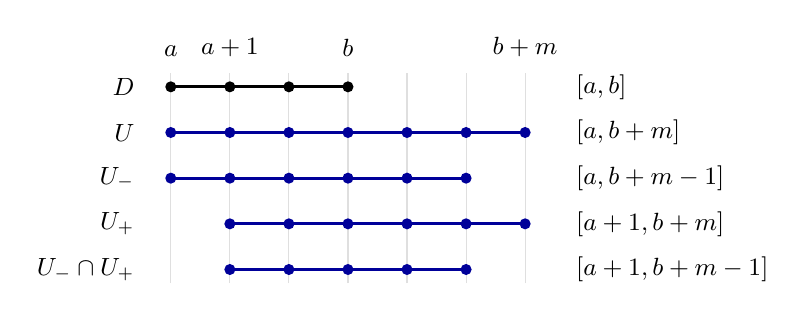
\begin{tikzpicture}[x=.75cm,y=.58cm,font=\small]
  \foreach \x in {0,...,6}
    \draw[gray!25] (\x,-.3)--(\x,4.3);
  \node[above] at (0,4.45) {$a$};
  \node[above] at (1,4.45) {$a+1$};
  \node[above] at (3,4.45) {$b$};
  \node[above] at (6,4.45) {$b+m$};
  \node[anchor=east] at (-.45,4) {$D$};
  \node[anchor=east] at (-.45,3) {$U$};
  \node[anchor=east] at (-.45,2) {$U_-$};
  \node[anchor=east] at (-.45,1) {$U_+$};
  \node[anchor=east] at (-.45,0) {$U_-\cap U_+$};
  \draw[very thick] (0,4)--(3,4);
  \draw[very thick,blue!60!black] (0,3)--(6,3);
  \draw[very thick,blue!60!black] (0,2)--(5,2);
  \draw[very thick,blue!60!black] (1,1)--(6,1);
  \draw[very thick,blue!60!black] (1,0)--(5,0);
  \foreach \x in {0,...,3} \fill (\x,4) circle (2pt);
  \foreach \x in {0,...,6} \fill[blue!60!black] (\x,3) circle (2pt);
  \foreach \x in {0,...,5} \fill[blue!60!black] (\x,2) circle (2pt);
  \foreach \x in {1,...,6} \fill[blue!60!black] (\x,1) circle (2pt);
  \foreach \x in {1,...,5} \fill[blue!60!black] (\x,0) circle (2pt);
  \node[anchor=west] at (6.7,4) {$[a,b]$};
  \node[anchor=west] at (6.7,3) {$[a,b+m]$};
  \node[anchor=west] at (6.7,2) {$[a,b+m-1]$};
  \node[anchor=west] at (6.7,1) {$[a+1,b+m]$};
  \node[anchor=west] at (6.7,0) {$[a+1,b+m-1]$};
\end{tikzpicture}
\caption{Occurrence intervals for one fixed base cell in Case~1,
illustrated with $b-a=m=3$.  Each point represents a translate of
that cell, not a copy of the domain $D$.  The formulas also apply
when $m=0$, with an interval empty if its lower endpoint exceeds
its upper endpoint.  In that case $U=D$, and the complete adjacent
overlap graphs are nonempty trees by Lemma~\ref{mag:tree-domain}.}
\label{mag:domain-intervals}
\end{figure}

If $m=0$, both adjacent overlaps are trees.  If $m\geq1$, the
interval calculation gives
\[
 U_- =\bigcup_{i=0}^{m-1}\tau^iD,
 \qquad
 U_+ =\bigcup_{i=1}^{m}\tau^iD.
\]
Minimality of $m$ shows that neither contains a closed lift of
$\lambda$.  Their intersection is
\[
 U_-\cap U_+=
 \begin{cases}
   D\cap\tau D,&m=1,\\
   \displaystyle\bigcup_{i=1}^{m-1}\tau^iD,&m\geq2.
 \end{cases}
\]
It is connected and nonempty.  In the case $m=0$, a tree cannot
contain the nontrivial immersed circuit, so the overlaps are
again Magnus subgraphs.
The lifted circuit has the same length as $\lambda$ and strictly
more support vertices.  Thus the first coordinate of
\eqref{mag:complexity} has decreased.

\smallskip\noindent
\emph{Case 2: the lifted support projects injectively on vertices.}
It then projects isomorphically onto $S_\lambda$:
two lifts of the same oriented edge cannot have the same initial
vertex.  The character therefore vanishes on
$\pi_1S_\lambda$, and every lift of this support is a copy of it.
Choose a spanning tree $T_S$ of $S_\lambda$ and extend it to a
spanning tree of $\Gamma$; in the resulting level coordinates
each support copy lies at one level.

Contract the support downstairs and every support copy upstairs.
This gives the connected cyclic cover of the quotient graph
$\Gamma/S_\lambda$ corresponding to the still-surjective
character.  Apply Lemma~\ref{mag:tree-domain} there.
Expand every occurrence of the contracted vertex in the resulting
domain by a copy of $T_S$.  At one chosen occurrence, add all the
remaining edges of $S_\lambda$.
Call the resulting graph $U$.  It is a connected domain:
the support-tree cells have the same occurrence interval as the
contracted vertex, and each added support edge has a singleton
occurrence interval.  The overlap $U\cap\tau U$ is a tree,
obtained by expanding vertices of a tree into trees; none of the
added support edges lies in it.  The full support at the chosen
occurrence contains a closed lift $\widetilde\lambda$.
Both overlaps are trees and hence Magnus subgraphs.

Here the first complexity coordinate is unchanged and the second
decreases.  To see this directly, for each base open cell its
number of occurrences in $U$ exceeds its number of occurrences
in $U\cap\tau U$ by one.  Counting vertices and edges gives
\[
 \chi(U)-\chi(U\cap\tau U)=\chi(\Gamma).
\]
Since the overlap is a tree, $\chi(U)=\chi(\Gamma)+1$, and hence
\[
 \operatorname{rank}\pi_1U
       =\operatorname{rank}\pi_1\Gamma-1.
\]

\smallskip\noindent
\emph{The HNN splitting.}
Both constructions now have the required overlaps and complexity
decrease.  We recover $X$ from the translates of $Z$, as in
\cite[Proposition~4.3]{LintonHierarchies2025}.  Since
$\phi([\lambda])=0$, the graph cover extends over the cells to
the cyclic cover $Y\to X$.  The translates $\tau^iZ$ cover $Y$,
and their two-cell interiors are distinct.
Form a line of disjoint copies of $Z$, joining each adjacent pair
by the cylinder on its intersection.  Denote this space by $W$;
collapsing these cylinders gives an equivariant map $W\to Y$.
For a finite interval of copies, the intersection of a newly
adjoined copy with the preceding union is precisely its adjacent
overlap.  Indeed, if a graph cell lies in the new copy and in an
earlier copy, its occurrence interval also puts it in the
immediately preceding copy.  Distinct copies have no common
two-cell interior, and cell boundaries consist of graph cells,
so this checks the entire intersection.
Van Kampen therefore shows inductively that the
cylinder-collapse map induces a fundamental-group isomorphism
over every finite interval.  Every loop and every homotopy uses
only finitely many copies, so $W\to Y$ induces an isomorphism on
fundamental groups as well.

Taking the quotient by translation gives a graph of spaces with
one vertex space $Z$ and one edge space, and a map
$W/\langle\tau\rangle\to X$.
The two covering exact sequences have quotient $\mathbb Z$;
the map is an isomorphism on their kernels and on this quotient.
It follows that it induces an isomorphism on fundamental groups.
The edge maps are injective by
Lemma~\ref{mag:graph-magnus}, because each overlap omits a
traversed relator edge.  Thus this graph of spaces gives the HNN
extension \eqref{mag:hnn}, and the normal form theorem gives
injection of $H$ into $\pi_1X$.

\smallskip\noindent
\emph{Simultaneous Magnus bases and the edge isomorphism.}
It remains to choose the two Magnus subsets simultaneously and
specify their basepoint paths.  If the overlap groups are trivial, this is
immediate.  Otherwise put $U_0=U_-\cap U_+$, which is connected
and nonempty by the construction.  Extend a spanning tree of
$U_0$ to spanning trees of $U_-$ and $U_+$.
Their intersection is exactly the chosen tree of $U_0$, so their
union is a tree.  Extend that union to a spanning tree of $U$.
With basepoint in $U_0$, the non-tree edges of the two overlaps
are then subsets of a single free basis of $\pi_1U$.
Their common letters freely generate $C=\pi_1U_0$, which is a
free factor in each side group.

To specify the stable letter in this nontrivial-edge case,
choose $x\in U_0$ and a path $q\subset U_+$ from $x$ to $\tau x$.
The latter vertex belongs to $U_+$ because $x\in U_-$.
Then $t=[p(q)]$ has height one, and the edge isomorphism sends a
loop $a$ in $U_-$ to $q\,(\tau a)\,q^{-1}$ in $U_+$.
Its projection is $tat^{-1}$, giving the specified isomorphism
in \eqref{mag:hnn}.
When the overlap groups are trivial, choose instead any
$x\in U_-$ and a path $q\subset U$ from $x$ to $\tau x$.
Again $t=[p(q)]$ has height one, and the edge relation is empty.
In either case, $q$ in the copy $Z$ closes in the quotient graph
of spaces by crossing the cylinder to the copy $\tau Z$ at
$\tau x$.  It crosses the quotient loop edge exactly once,
so it is a stable letter; collapsing the cylinder sends it to
$p(q)$.

Finally, $\pi_1U$ injects into $\pi_1\Gamma$, by inclusion into
the graph cover and its covering map.  If the lifted relator
were a proper power in $\pi_1U$, its image would be a proper
power in $\pi_1\Gamma$.  This proves the remaining assertion.
\end{proof}

\subsection{Hyperbolicity and the final reductions}

The preceding construction supplies the geometric input to the
combination theorem.  We now check its algebraic hypotheses.

\begin{proposition}\label{mag:nonpower-hyperbolicity}
Let $\Gamma$ be a finite connected graph, and let
$\lambda\colon S^1\to\Gamma$ be a nontrivial immersed circuit
representing a non-power in $\pi_1\Gamma$.
If $\pi_1(\Gamma\cup_\lambda D^2)$ is $BS$-free, then it is
word-hyperbolic.
\end{proposition}

\begin{proof}
We induct on the nonnegative lexicographic complexity
\eqref{mag:complexity}.  In graph rank one, the non-power relator
generates the infinite cyclic fundamental group, and the quotient
is trivial.  Rank zero cannot support the stipulated circuit.

In higher rank, apply Lemma~\ref{mag:splitting} to obtain
\[
 G=\langle H,t\mid tAt^{-1}=B\rangle.
\]
The vertex group $H$ embeds in $G$, and so is $BS$-free.
It has a non-power graph presentation of smaller complexity,
hence is hyperbolic by induction.  The one-relator torsion
theorem makes it torsion-free
\cite[Theorem~2]{McCoolSchupp1973}.
The side groups $A$ and $B$ are finitely generated free Magnus
subgroups of $H$; by
\cite[Theorem~4.7]{LintonHyperbolic2026}, they are quasiconvex in
$H$.

Use the simultaneous bases from Lemma~\ref{mag:splitting}.
Collins's conjugate-intersection theorem
\cite[Theorem~2]{Collins2008Conjugates}, which permits equal
Magnus subgroups, says that for $M,N\in\{A,B\}$ and $g\in H$,
\[
 M\cap gNg^{-1}\text{ noncyclic}\quad\Longrightarrow\quad g\in MN.
\]
This is the first overlap hypothesis of
Theorem~\ref{ann:combination}.
Collins's direct-intersection theorem
\cite[Theorem~1]{Collins2008Conjugates} gives
\[
 I=A\cap B=C\quad\text{or}\quad I=C*\langle u\rangle,
\]
where $C$ is generated by the common basis letters and the
second expression is an internal free product with an infinite
cyclic group.  Thus $I$ and its transported copy $J=t^{-1}It$
are finitely generated.
If the edge group is nontrivial, the two Magnus subgraphs
$U_-,U_+$ have connected intersection by the construction.
Linton's strong-inertia lemma
\cite[Lemma~2.10]{LintonHierarchies2025} states that the
intersection of the fundamental groups of two such Magnus
subgraphs is strongly inert in either side group.
It follows that $I$ is strongly inert in $P=A$ and in $B$.
Isomorphisms preserve reduced ranks and the indexing double
cosets, so transporting the latter assertion through the edge
isomorphism makes $J$ strongly inert in $P$ as well.
These are precisely the two strong reduced-rank inertia
inequalities in Theorem~\ref{ann:combination}.
When the edge group is trivial, the same requirements hold
directly.

All hypotheses of Theorem~\ref{ann:combination} have now been
verified.  Its conclusion makes $G$ hyperbolic, completing the
induction.
\end{proof}

\begin{proof}[Proof of Theorem~\ref{thm:main}]
Freely and cyclically reduce the defining relator; conjugating or
inverting it does not change its normal closure.
If it becomes trivial, the group is a finitely generated free
group and is hyperbolic.

If the cyclically reduced relator is a proper power, write it as
$w^k$, where $w$ is a nontrivial cyclically reduced non-power and
$k\geq2$.  Newman's spelling theorem
\cite{Newman1968}, in the form
\cite[Theorem~4]{McCoolSchupp1973}, says that every nonempty
freely reduced null word contains a segment of a cyclic conjugate
of $w^{\pm k}$ of length greater than $(k-1)|w|$.
This is strictly more than half the relator length, including
when $k=2$.  Replacing that segment by the inverse complementary
segment strictly shortens the word and uses one defining
relation.  Repeating, with free reduction after each replacement,
fills a null word with at most its original length in relator
cells.  These shortening rules give a finite Dehn presentation
(and a linear isoperimetric inequality).  The group is therefore
word-hyperbolic
\cite[Theorem~III.$\Gamma$.2.6]{BridsonHaefliger1999}.

In the remaining case, realize the cyclically reduced non-power
relator as an immersed circuit in the basis rose.
Proposition~\ref{mag:nonpower-hyperbolicity} applies and proves
hyperbolicity under the stated exclusion of $BS(m,n)$ for all
nonzero integers $m,n$.
\end{proof}

\begin{proof}[Proof of Theorem~\ref{thm:magnus}]
Under its non-power graph-presentation hypotheses,
Proposition~\ref{mag:nonpower-hyperbolicity} makes the ambient
group hyperbolic.  For any connected subgraph omitting a
traversed edge, Lemma~\ref{mag:graph-magnus} identifies its
fundamental group with an injective Magnus subgroup in a
one-relator presentation.  Linton's theorem
\cite[Theorem~4.7]{LintonHyperbolic2026} makes that subgroup
quasiconvex.  Basepoint paths only conjugate it, so the assertion
holds for every choice of such paths.
\end{proof}

\section{Virtual free-by-cyclic consequence}\label{sec:free-by-cyclic}

We now combine the hyperbolicity theorem with the companion virtual
compact specialness theorem and the results of Kielak--Linton.

\begin{corollary}\label{cor:free-by-cyclic}
Let $X$ be finite, let $r\in F(X)$, and suppose that
$G=F(X)/\langle\!\langle r\rangle\!\rangle$ contains no subgroup
isomorphic to $\operatorname{BS}(m,n)$ for any nonzero integers $m,n$.
There are a finite-index subgroup $H\leq G$, an integer $d\geq0$, an
automorphism $\alpha$ of the rank-$d$ free group $F_d$, and an embedding
\[
H\hookrightarrow F_d\rtimes_\alpha\mathbb Z.
\]
Consequently the same $H$ fits into an exact sequence
\[
1\longrightarrow K\longrightarrow H\longrightarrow Q\longrightarrow1,
\qquad K\text{ free},\quad Q\leq\mathbb Z.
\]
Thus $G$ is virtually free-by-cyclic, with the rank of $K$ allowed to be
infinite and $Q$ allowed to be trivial.
\end{corollary}

\begin{proof}
If $G$ is finite, take $H=1$ and $F_d=F_0=1$, with ambient group
$\mathbb Z$. Otherwise Theorem~\ref{thm:main} makes $G$ hyperbolic,
and Theorem~1.1 of \cite{OpenAIVirtualSpecialness} makes it virtually
compact special. The free group $F(X)$ is the fundamental group of a
compact connected planar surface with $|X|+1$ boundary components.
Kielak--Linton's Corollary~1.3
\cite{KielakLinton2024Virtually} therefore makes $G$ virtually
free-by-cyclic. The surface may be a disk, and their relator is
arbitrary; trivial relators and proper powers are not excluded.

For a hyperbolic virtually compact special group, Theorem~1.1 of
\cite{KielakLinton2024Virtually} equates being virtually free-by-cyclic
with a finite-index embedding in a free-by-cyclic group with finitely
generated free kernel. In the
rational cohomological dimension two branch of their proof the ambient
quotient is $\mathbb Z$. In the dimension-at-most-one branch they
obtain a finite-index free subgroup, which has finite rank here and
embeds in its direct product with $\mathbb Z$. In either branch the
ambient extension splits over $\mathbb Z$, giving the displayed
semidirect product.

Identify $H$ with its image and restrict the projection onto
$\mathbb Z$. Its kernel is $K=H\cap F_d$, which is free as a subgroup
of a free group, and its image is a subgroup $Q\leq\mathbb Z$. This is
the asserted exact sequence. Finite generation of the ambient kernel
$F_d$ does not imply finite generation of $K$.
\end{proof}

The companion also proves that
\[
F*_\phi=\langle F,t\mid t^{-1}ft=\phi(f)\ (f\in F)\rangle
\]
is virtually compact special whenever $F$ is free of finite rank,
$\phi:F\to F$ is injective, and $F*_\phi$ is word-hyperbolic
\cite[Theorem~1.2]{OpenAIVirtualSpecialness}. Such a group is finitely
generated, so Kielak--Linton's Corollary~1.8
\cite{KielakLinton2024Virtually}, followed by the same ambient argument,
gives the finite-index embedding and subgroup-closed free-by-cyclic
conclusion for these ascending HNN extensions as well. The resulting
free kernel is not asserted to be their canonical height kernel.

\bibliographystyle{plain}
\bibliography{references}
\end{document}
